\section{Additional Figures}
\label{sec:appendix1:add_figures}

\begin{figure}[t!]
  \begin{center}
    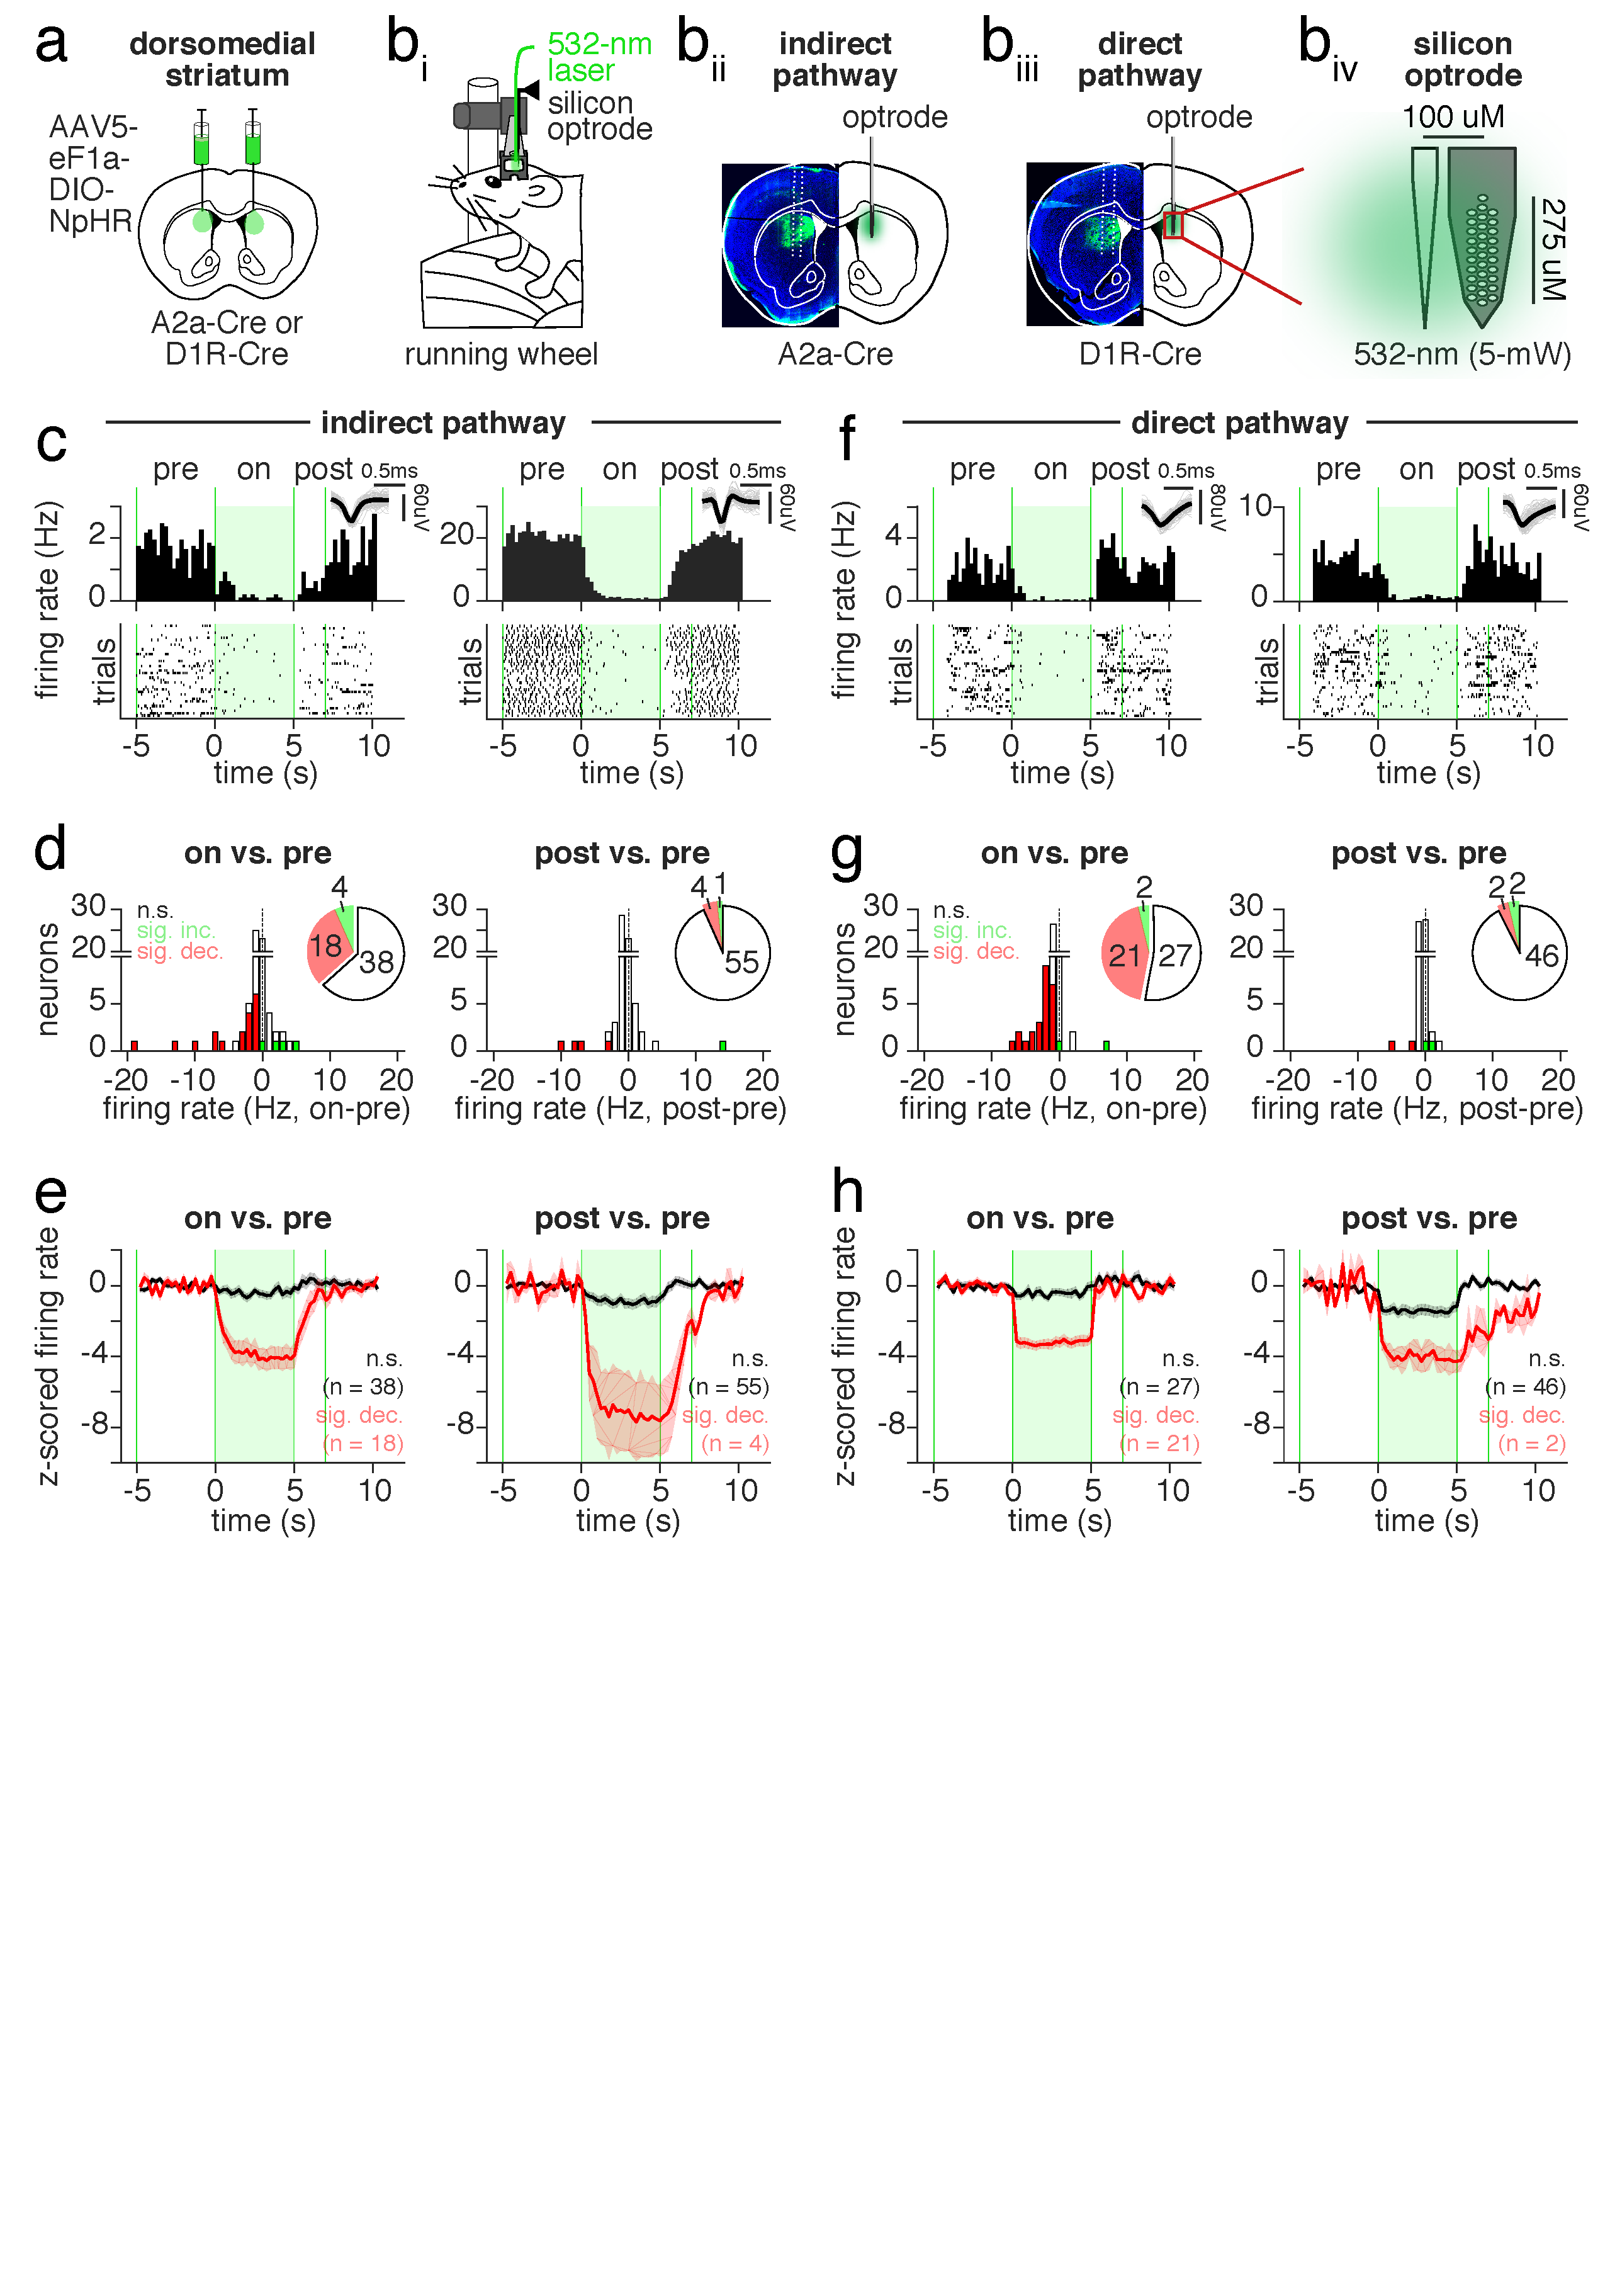
\includegraphics[width=0.90\linewidth]{ch7-appendix1/appendix1-figures/ExtData_Fig1.pdf}
    \caption[Optogenetic inhibition of DMS pathways is effective, generating little post-inhibitory rebound, nor excitation during the inhibition period]{\textbf{Optogenetic inhibition of DMS pathways is effective, generating little post-inhibitory rebound, nor excitation during the inhibition period.} (a) Schematic of viral delivery of AAV5-eF1a-DIO-NpHR to the dorsomedial striatum (DMS) of A2a-Cre or D1R-Cre mice. (b,i) Schematic of electrophysiological recording and laser delivery (532-nm, 5-mW) to the DMS in awake, head-fixed mice ambulating on a running wheel. (b,ii) Example recording electrode tracks and cre-dependent NpHR expression in an A2a-Cre mouse targeting the indirect pathway of the DMS. (b,iii) As in b,ii but in a D1R-Cre mouse targeting the DMS direct pathway. (b,iv) Schematic of silicon optrode recording tip, including tapered optical fiber coupled to a 32-channel silicon probe. (c) Two example peristimulus time histograms (PSTH) (top) and raster plots of trial-by-trial spike times (bottom) from single neurons recorded from the DMS of an A2a-Cre mouse. Inset at top displays average spike waveform (black) and 100 randomly sampled spike waveforms (grey) for each neuron. A trial consisted of 5-s without laser (pre, -5 to 0-s), 5-s of 532-nm light (5-mW) delivery (on, 0 to 5-s), followed by a 10-s ITI (40 trials per recording site). The first 2-s following laser offset (post, 5-7-s) was used to assess post-inhibitory effects. (d) Left: Histogram of change in average firing rate (on-pre, Hz) for all neurons (n = 60) recorded from the DMS of A2a-Cre mice (n = 3). Colors indicate non-significant (black, n = 38 neurons), significantly decreased }
    \label{fig:ap1:ext1}
  \end{center}
  \vspace{-1.5cm}
\end{figure}
\begin{figure}[t!]
\vspace{-4cm}
  \contcaption{(red, n = 18 neurons) or increased (green, n = 4 neurons) changes in firing rate determined via paired, two-tailed signrank comparison of average across-trial baseline (pre) or laser (on) firing rates. A Bonferroni-corrected significance threshold was used to account for multiple neuron comparisons (p < 0.00083, or p = 0.05/60 neuron comparisons). Right: same as left but for change in firing rate (post-pre, Hz): non-significant (n = 55 neurons), significantly decreased (n = 4) or increased (n = 1). Insets display pie-chart summaries of the proportion of non-significant (black unfilled), significantly decreased (red) or increased (green) neurons. (e) Left: Mean $\pm$ SEM z-scored firing rate across all non-significantly modulated on vs pre (black, n = 38) or significantly decreased on vs pre (red, n = 18) neurons recorded from A2a-Cre mice. Right: same as left but for all non-significantly modulated post vs pre (black, n = 55) or significantly decreased post vs pre (red, n = 4) neurons. (f) Same as c but for example neurons recorded from the DMS of D1R-Cre mice. (g) Same as d but for all neurons (n = 50) recorded from the DMS of D1R-Cre mice (n = 2). Left (on-pre): non-significant (n = 27), significantly decreased (n = 21), or increased (n = 2). Right (post-pre): non-significant (n = 46), significantly decreased (n = 2) or increased (n = 2). A Bonferroni-corrected significance threshold was used to account for multiple neuron comparisons (p < 0.001, or p = 0.05/50 neuron comparisons). (h) same as e but for neurons recorded from the DMS of D1R-Cre mice.}% Continued caption
\end{figure}

\begin{figure}[t!]
  \begin{center}
    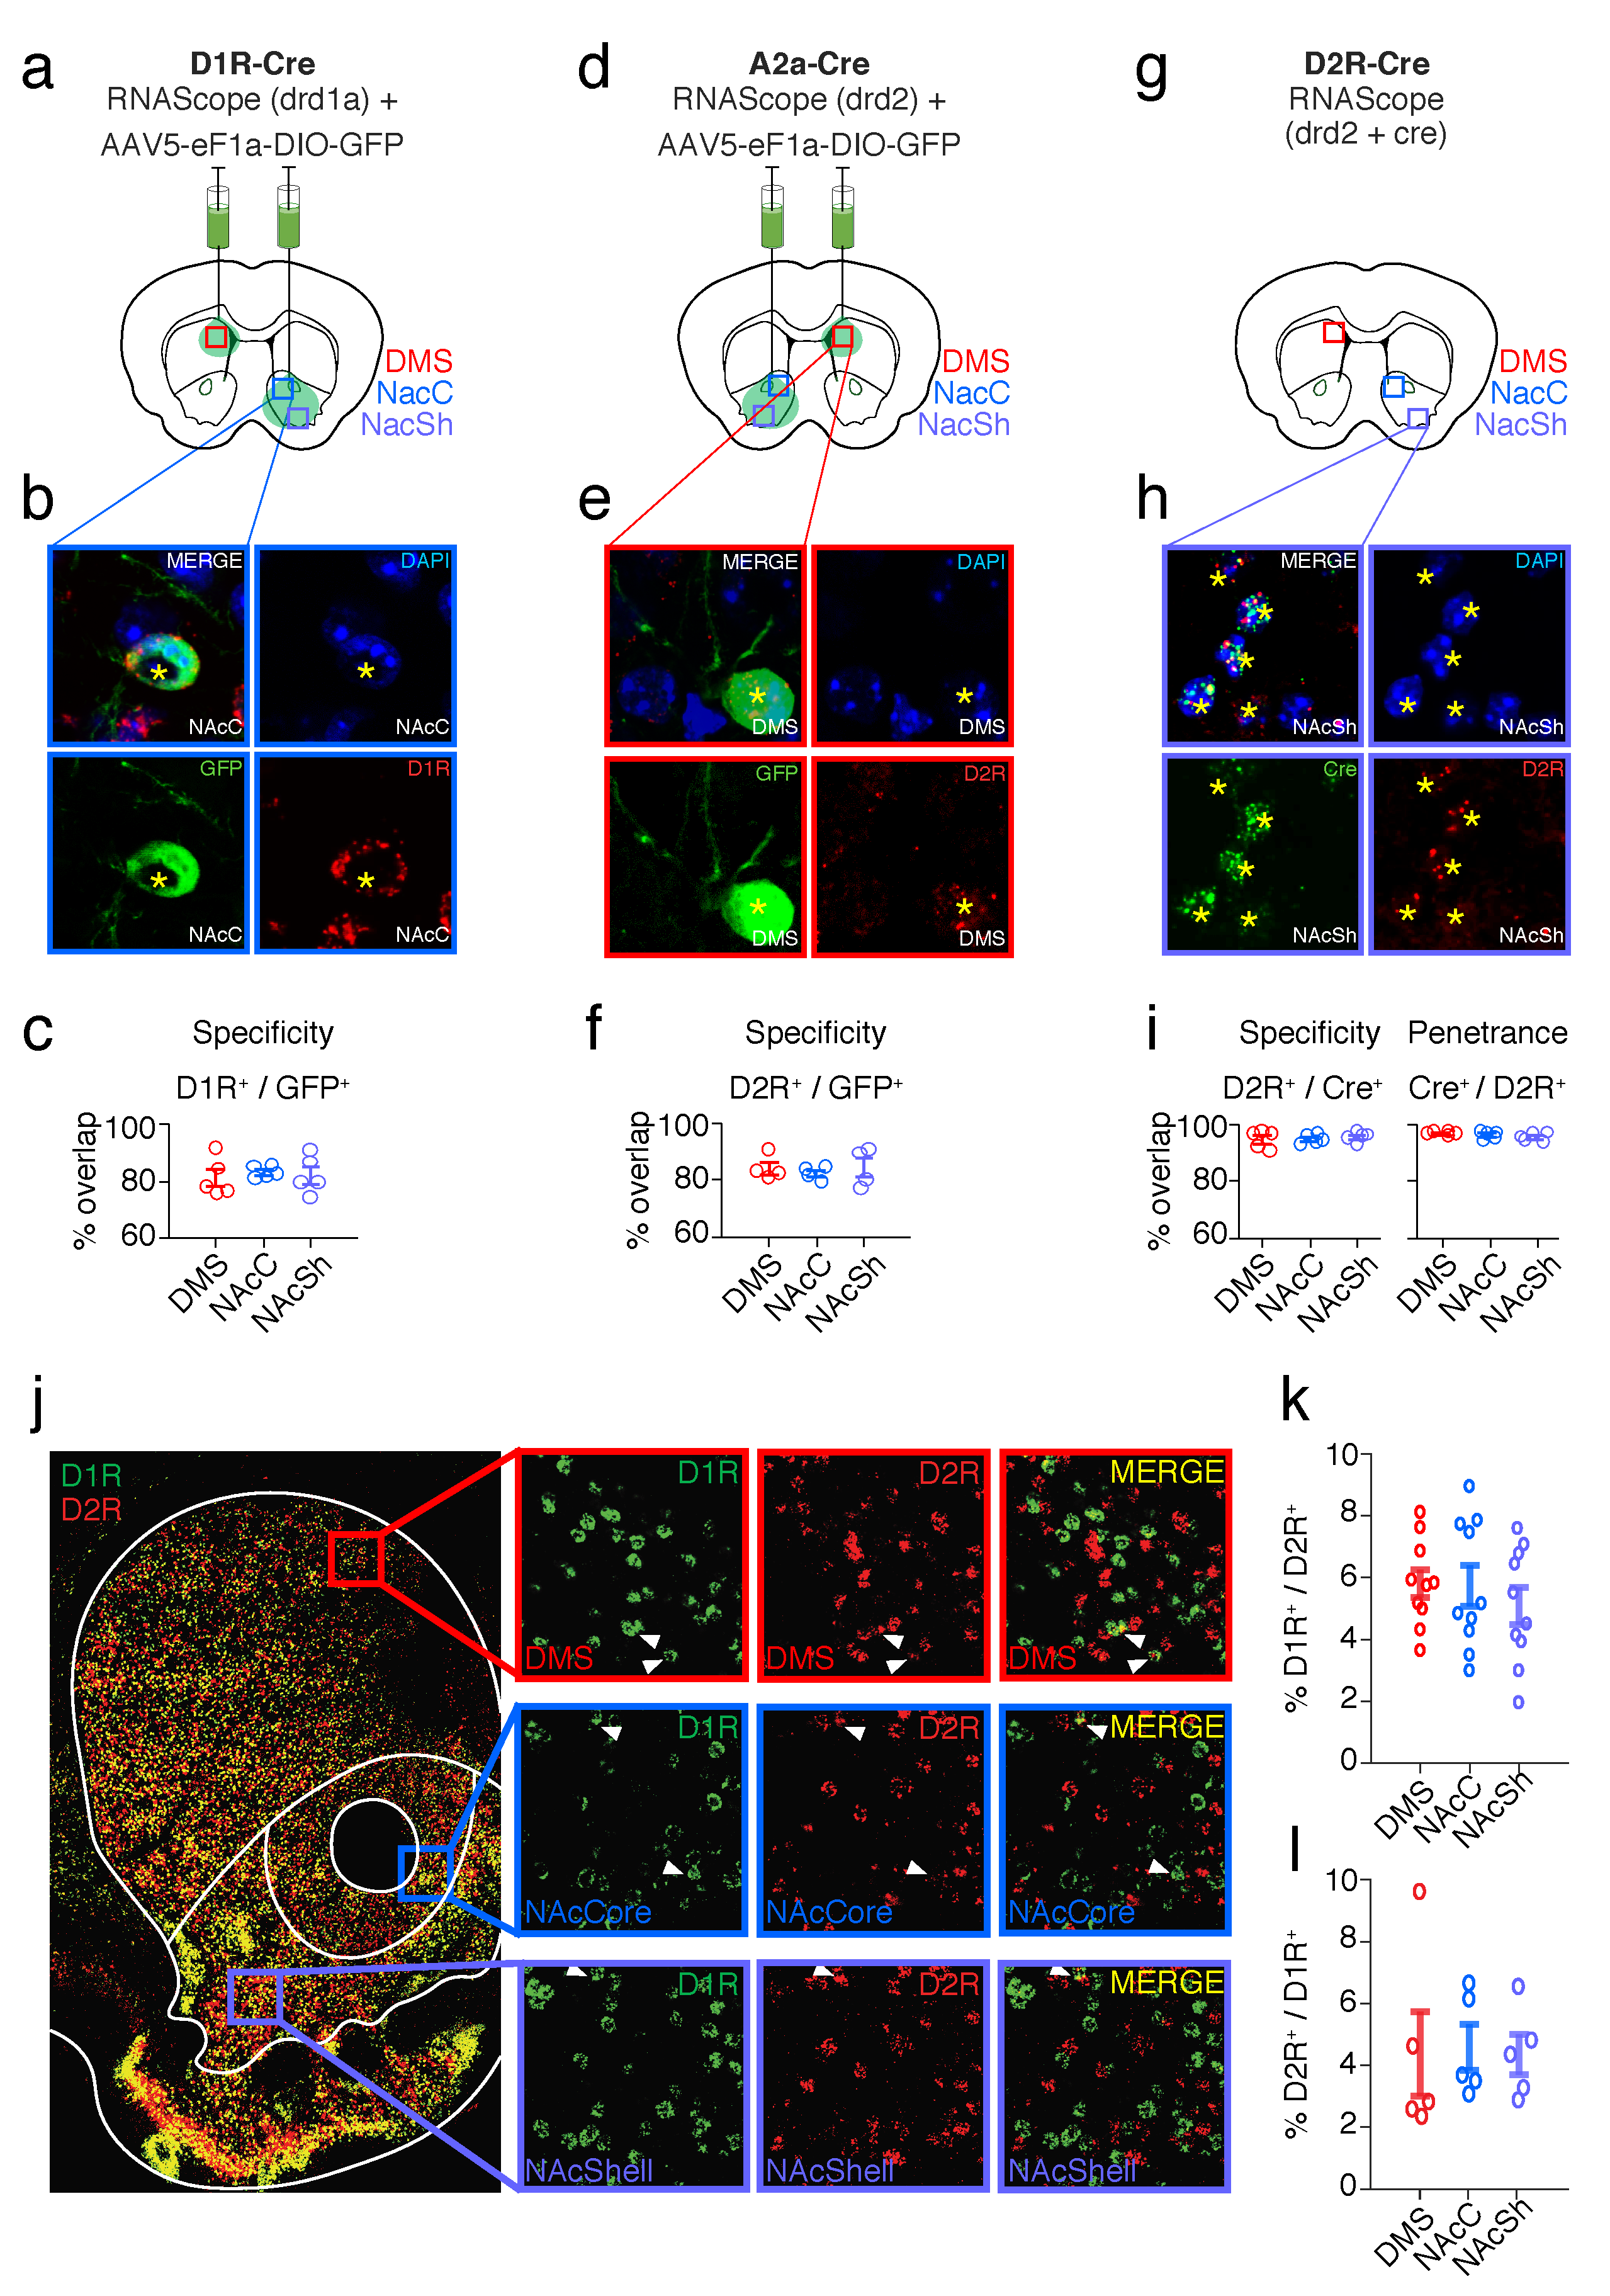
\includegraphics[width=0.85\linewidth]{ch7-appendix1/appendix1-figures/Supplementary_Fig1.pdf}
    \caption[Transgenic mouse lines faithfully report indirect and direct pathways across striatal subregions]{\textbf{Transgenic mouse lines faithfully report indirect and direct pathways across striatal subregions.}}
    \label{fig:ap1:supp1}
  \end{center}
  \vspace{-1.5cm}
\end{figure}
\begin{figure}[t!]
  \contcaption{(a) Schematic of viral delivery of AAV5-eF1a-DIO-GFP to the dorsomedial striatum (DMS) or nucleus accumbens (NAc) on opposite hemispheres of D1R-Cre mice. Red, blue, and purple squares denote representative areas for stereological quantification of viral co-expression with a drd1 mRNA probe (RNAScope) in the DMS, NAc core (NAcC), or NAc shell (NAcSh), respectively. (b) Example fluorescent confocal image (63x objective, 5x digital zoom) of the NAc core from a D1R-Cre mouse displaying virally- expressed GFP (green), drd1 mRNA (red), and DAPI (blue). (c) Percentage of GFP+ neurons co-expressing drd1 mRNA from 2 D1R-Cre mice across the DMS (red; n = 5 sections; 193 GFP+ neurons), NAcC (blue; n = 5 sections; 298 GFP+ neurons), or NacSh (purple; n = 4 sections; 312 GFP+ neurons). (d) Same as a, but for quantification of viral co-expression with a drd2 mRNA probe in A2a-Cre mice. (e) Same as b, but for an example image of the DMS from an A2a-Cre mouse and displaying drd2 mRNA (red). (f) Same as c, but for percentage of virally-expressed GFP+ neurons co-expressing drd2 mRNA in 2 A2a-Cre mice across the DMS (red; n = 4 sections; 312 GFP+ neurons), NAcC (blue; n = 4 sections; 326 GFP+ neurons), or NacSh (purple; n = 4 sections; 312 GFP+ neurons). (G) Same as A and D, but for quantification of co-expression of drd2 and cre mRNA in 2 D2R-Cre mice. (h) Same as b and e, but for an example image of the NAcSh from a D2R-Cre mouse and displaying cre mRNA (green) and drd2 mRNA (red). (i) Left: same as c and f, but for percentage of neurons with cre mRNA co-expressing drd2 mRNA in 2 D2R-Cre mice across the DMS (red; n = 5 sections; 1302 cre+ neurons), NAcC (blue; n = 5 sections; 1,104 cre+ neurons), or NacSh (purple; n = 4 sections; 1,187 cre+ neurons). Right: same as left but for neurons with drd2 mRNA co-expressing cre mRNA across DMS (red; n = 5 sections; 1,269 drd2+ neurons), NAcC (blue; n = 5 sections; 1,055 drd2+ neurons), or NacSh (purple; n = 5 sections; 1,114 cre+ neurons). Solid bars denote mean and s.e.m. throughout. (j) Example fluorescent confocal microscopy image of a coronal section from a DR2-Cre mouse that underwent fluorescent in situ hybridization with probes targeting drd1a and drd2 receptor mRNA. Left: 20x magnification tilescan spanning dorsal and ventral striatum. Right top: 63x confocal images of dorsomedial striatum (DMS, red square) and expression of drd1a mRNA (green), drd2 mRNA (red), and merged image of both (yellow). White triangles indicate co-expression of receptor probes in single neurons. Right middle: same as right top but for 63x confocal images of nucleus accumbens core (NAcC, blue square). Right bottom: same as right top but for 63x confocal images of nucleus accumbens shell (NAcSh, purple square). (k) Percentage of drd2+ neurons co-expressing drd1a mRNA from 2 D2R-Cre and 2 D1R-tdTomato mice in the DMS (red; n = 10 sections; 2,423 drd2+ neurons), NAcC (blue; n = 10 sections; 2,196 drd2+ neurons), or NacSh (purple; n = 10 sections; 2,220 drd2+ neurons). Circles indicate mean overlap from individual sections. (l) Same as k, but for percentage of drd1a+ neurons co-expressing drd2 mRNA from 2 D1R-tdTomato mice in the DMS (red; n = 5 sections; 868 drd1a+ neurons), NAcC (blue; n = 5 sections; 834 drd1a+ neurons), or NacSh (purple; n = 5 sections; 874 drd1a+ neurons). Throughout solid bars reflect mean $\pm$ S.E.M. and transparent ‘o’ denote individual slice mean. Each staining was repeated on 2 independent samples (mice) per group with similar results.  }% Continued caption
\end{figure}

\begin{figure}[t!]
  \begin{center}
    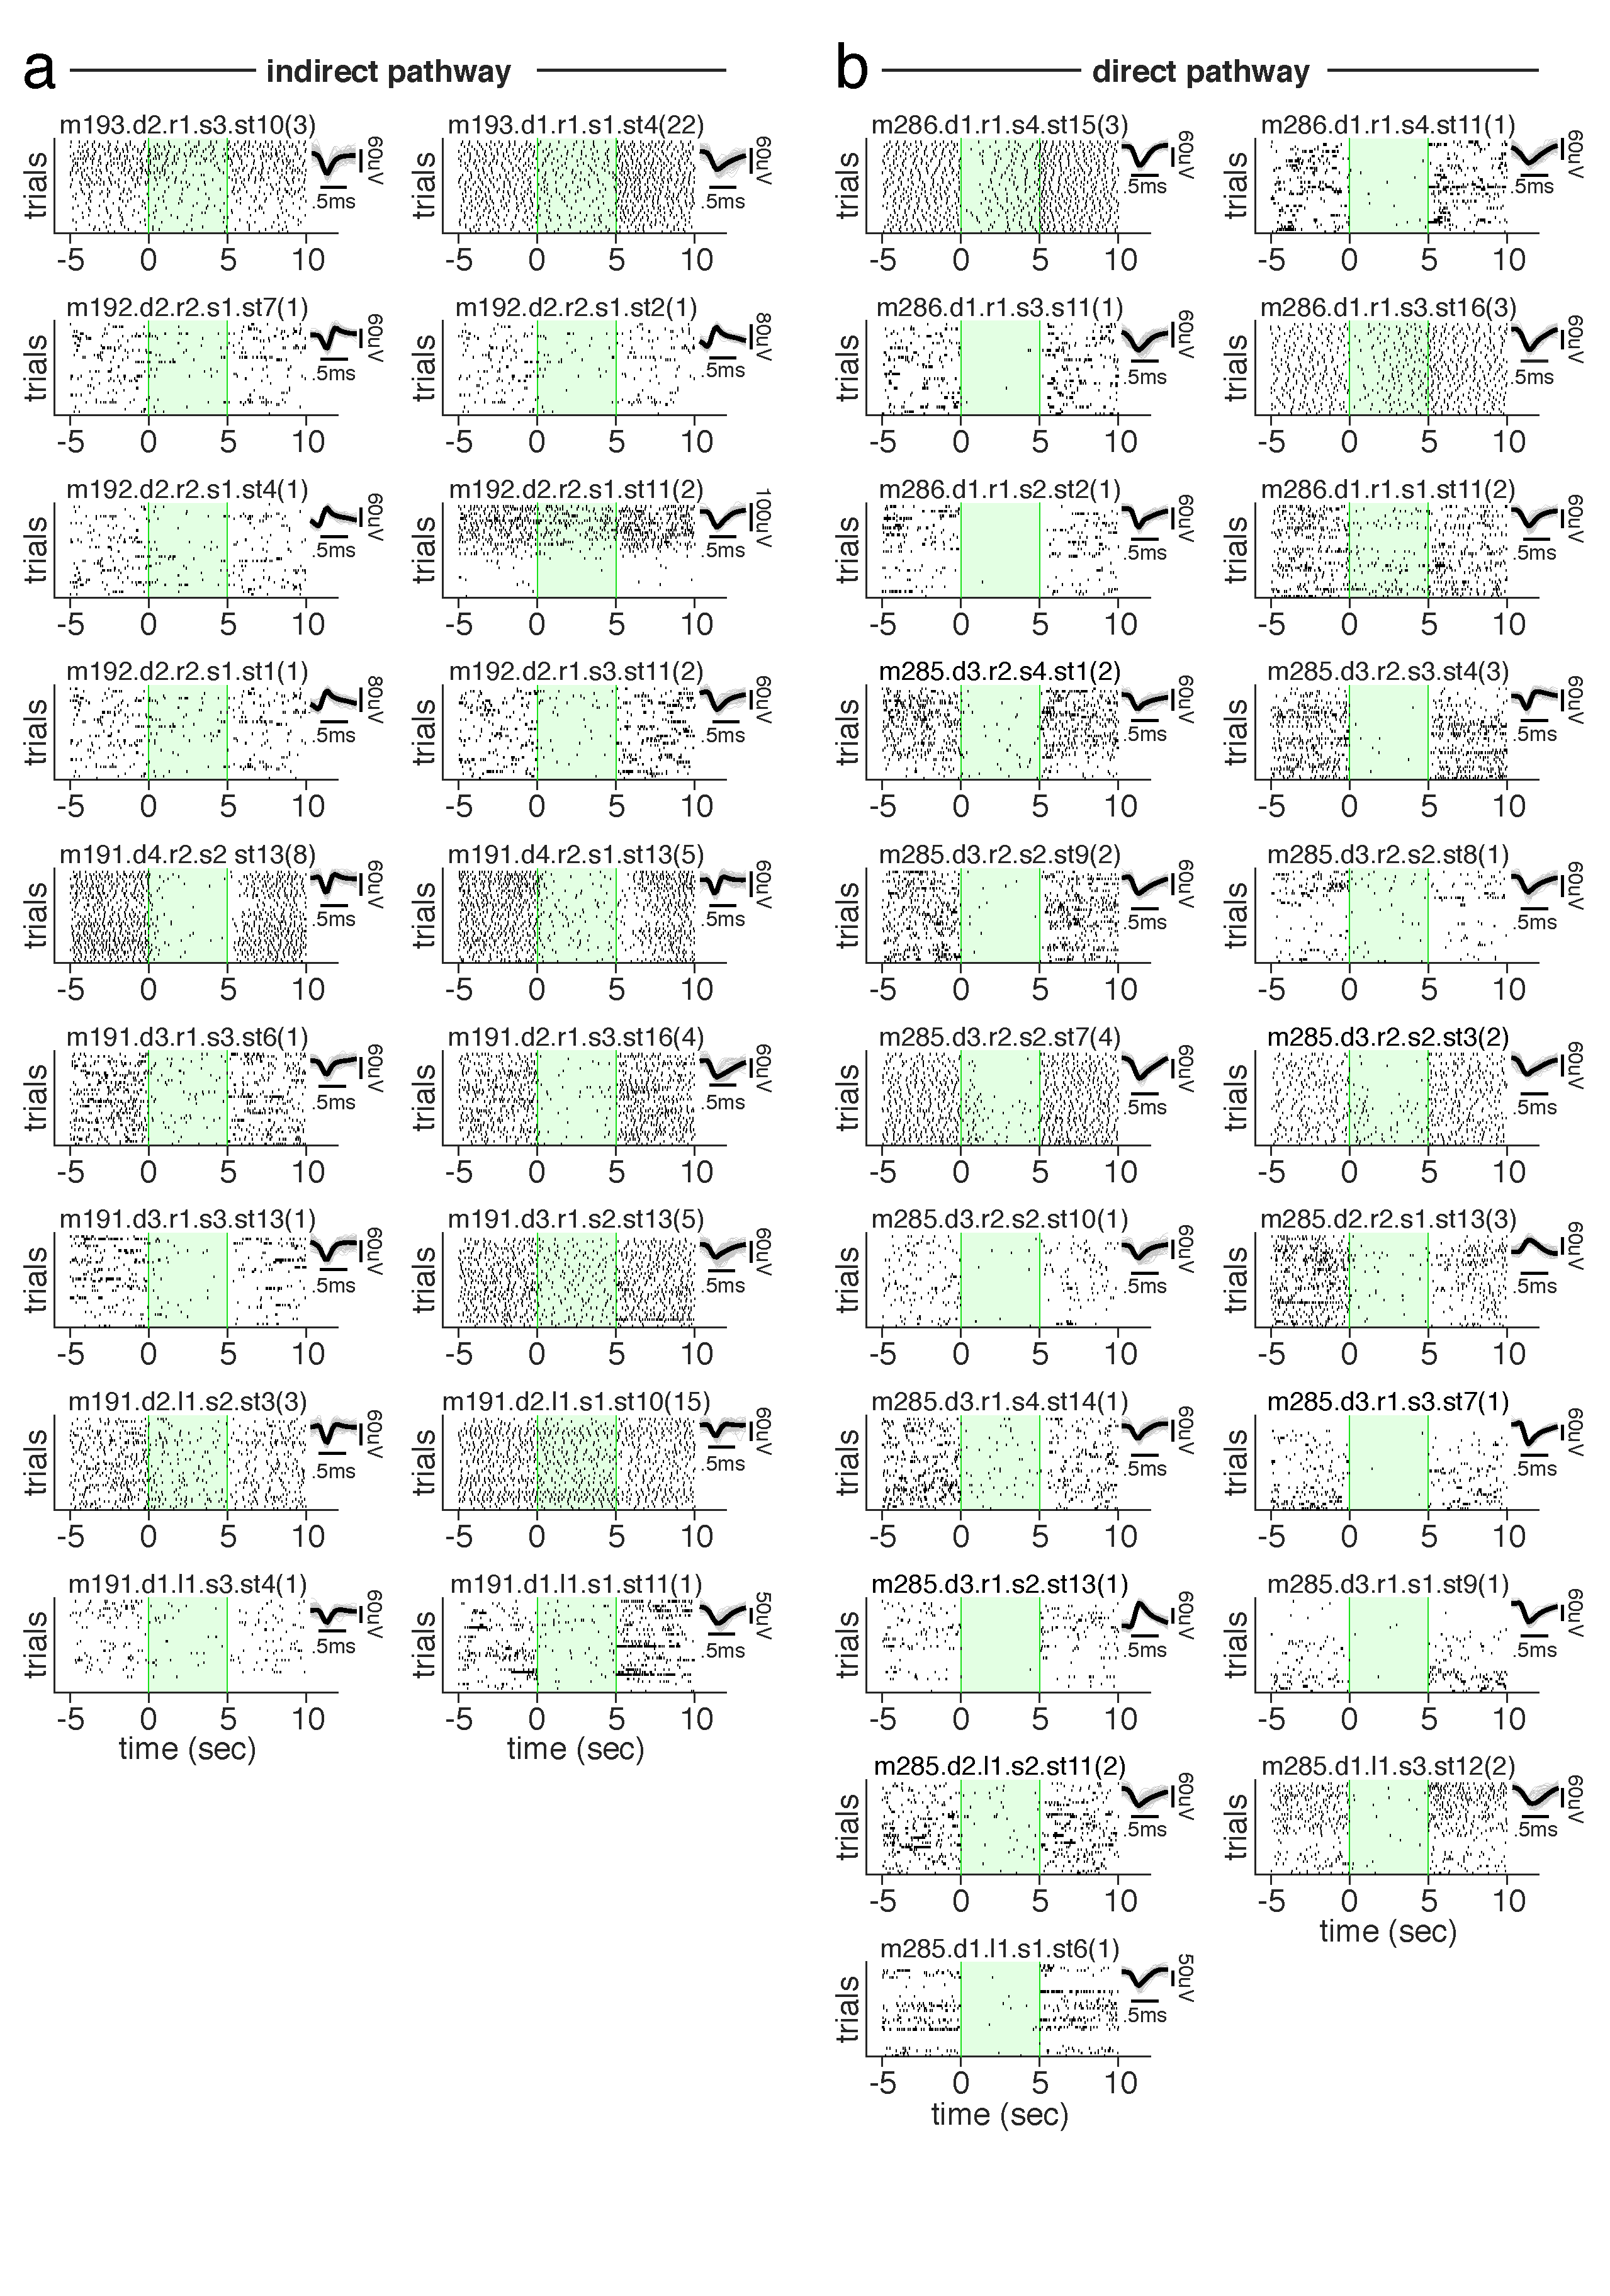
\includegraphics[width=0.90\linewidth]{ch7-appendix1/appendix1-figures/Supplementary_Fig2.pdf}
    \caption[Indirect and direct pathway inhibition of the DMS is stable across time]{\textbf{Indirect and direct pathway inhibition of the DMS is stable across time.} }
    \label{fig:ap1:supp2}
  \end{center}
  \vspace{-1.5cm}
\end{figure}
\begin{figure}[t!]
%\vspace{-3cm}
  \contcaption{\textbf{}  (a) Trial-by-trial raster plots of single neuron spiking during laser off baseline (-5 to 0s), 532-nm  (5-mW)  laser delivery (0 to 5s), and post laser offset (5 to 10s) for all significantly inhibited neurons  (n = 18/60) recorded from A2a-Cre mice expressing Cre-dependent NpHR in the DMS. 40 total trials of laser sweeps per recording site (~15 minutes), ordered in time top to bottom. Individual neuron labels indicate: m (mouse), d (day of recording), r/l (right/left hemisphere and penetration number), s (site or depth of recording probe numbered ventral to dorsal), and st (probe stereotrode channel). Number in parenthesis indicates the number of spikes sub-sampled for display. Inset displays average (bold) and 100 randomly sampled spike waveforms (grey). (b) As in a but for all significantly inhibited neurons recorded from D1R-Cre mice expressing Cre-dependent NpHR in the DMS (n =21/50).}% Continued caption
\end{figure}
\begin{figure}[t!]
\vspace{-2.5cm}
  \begin{center}
    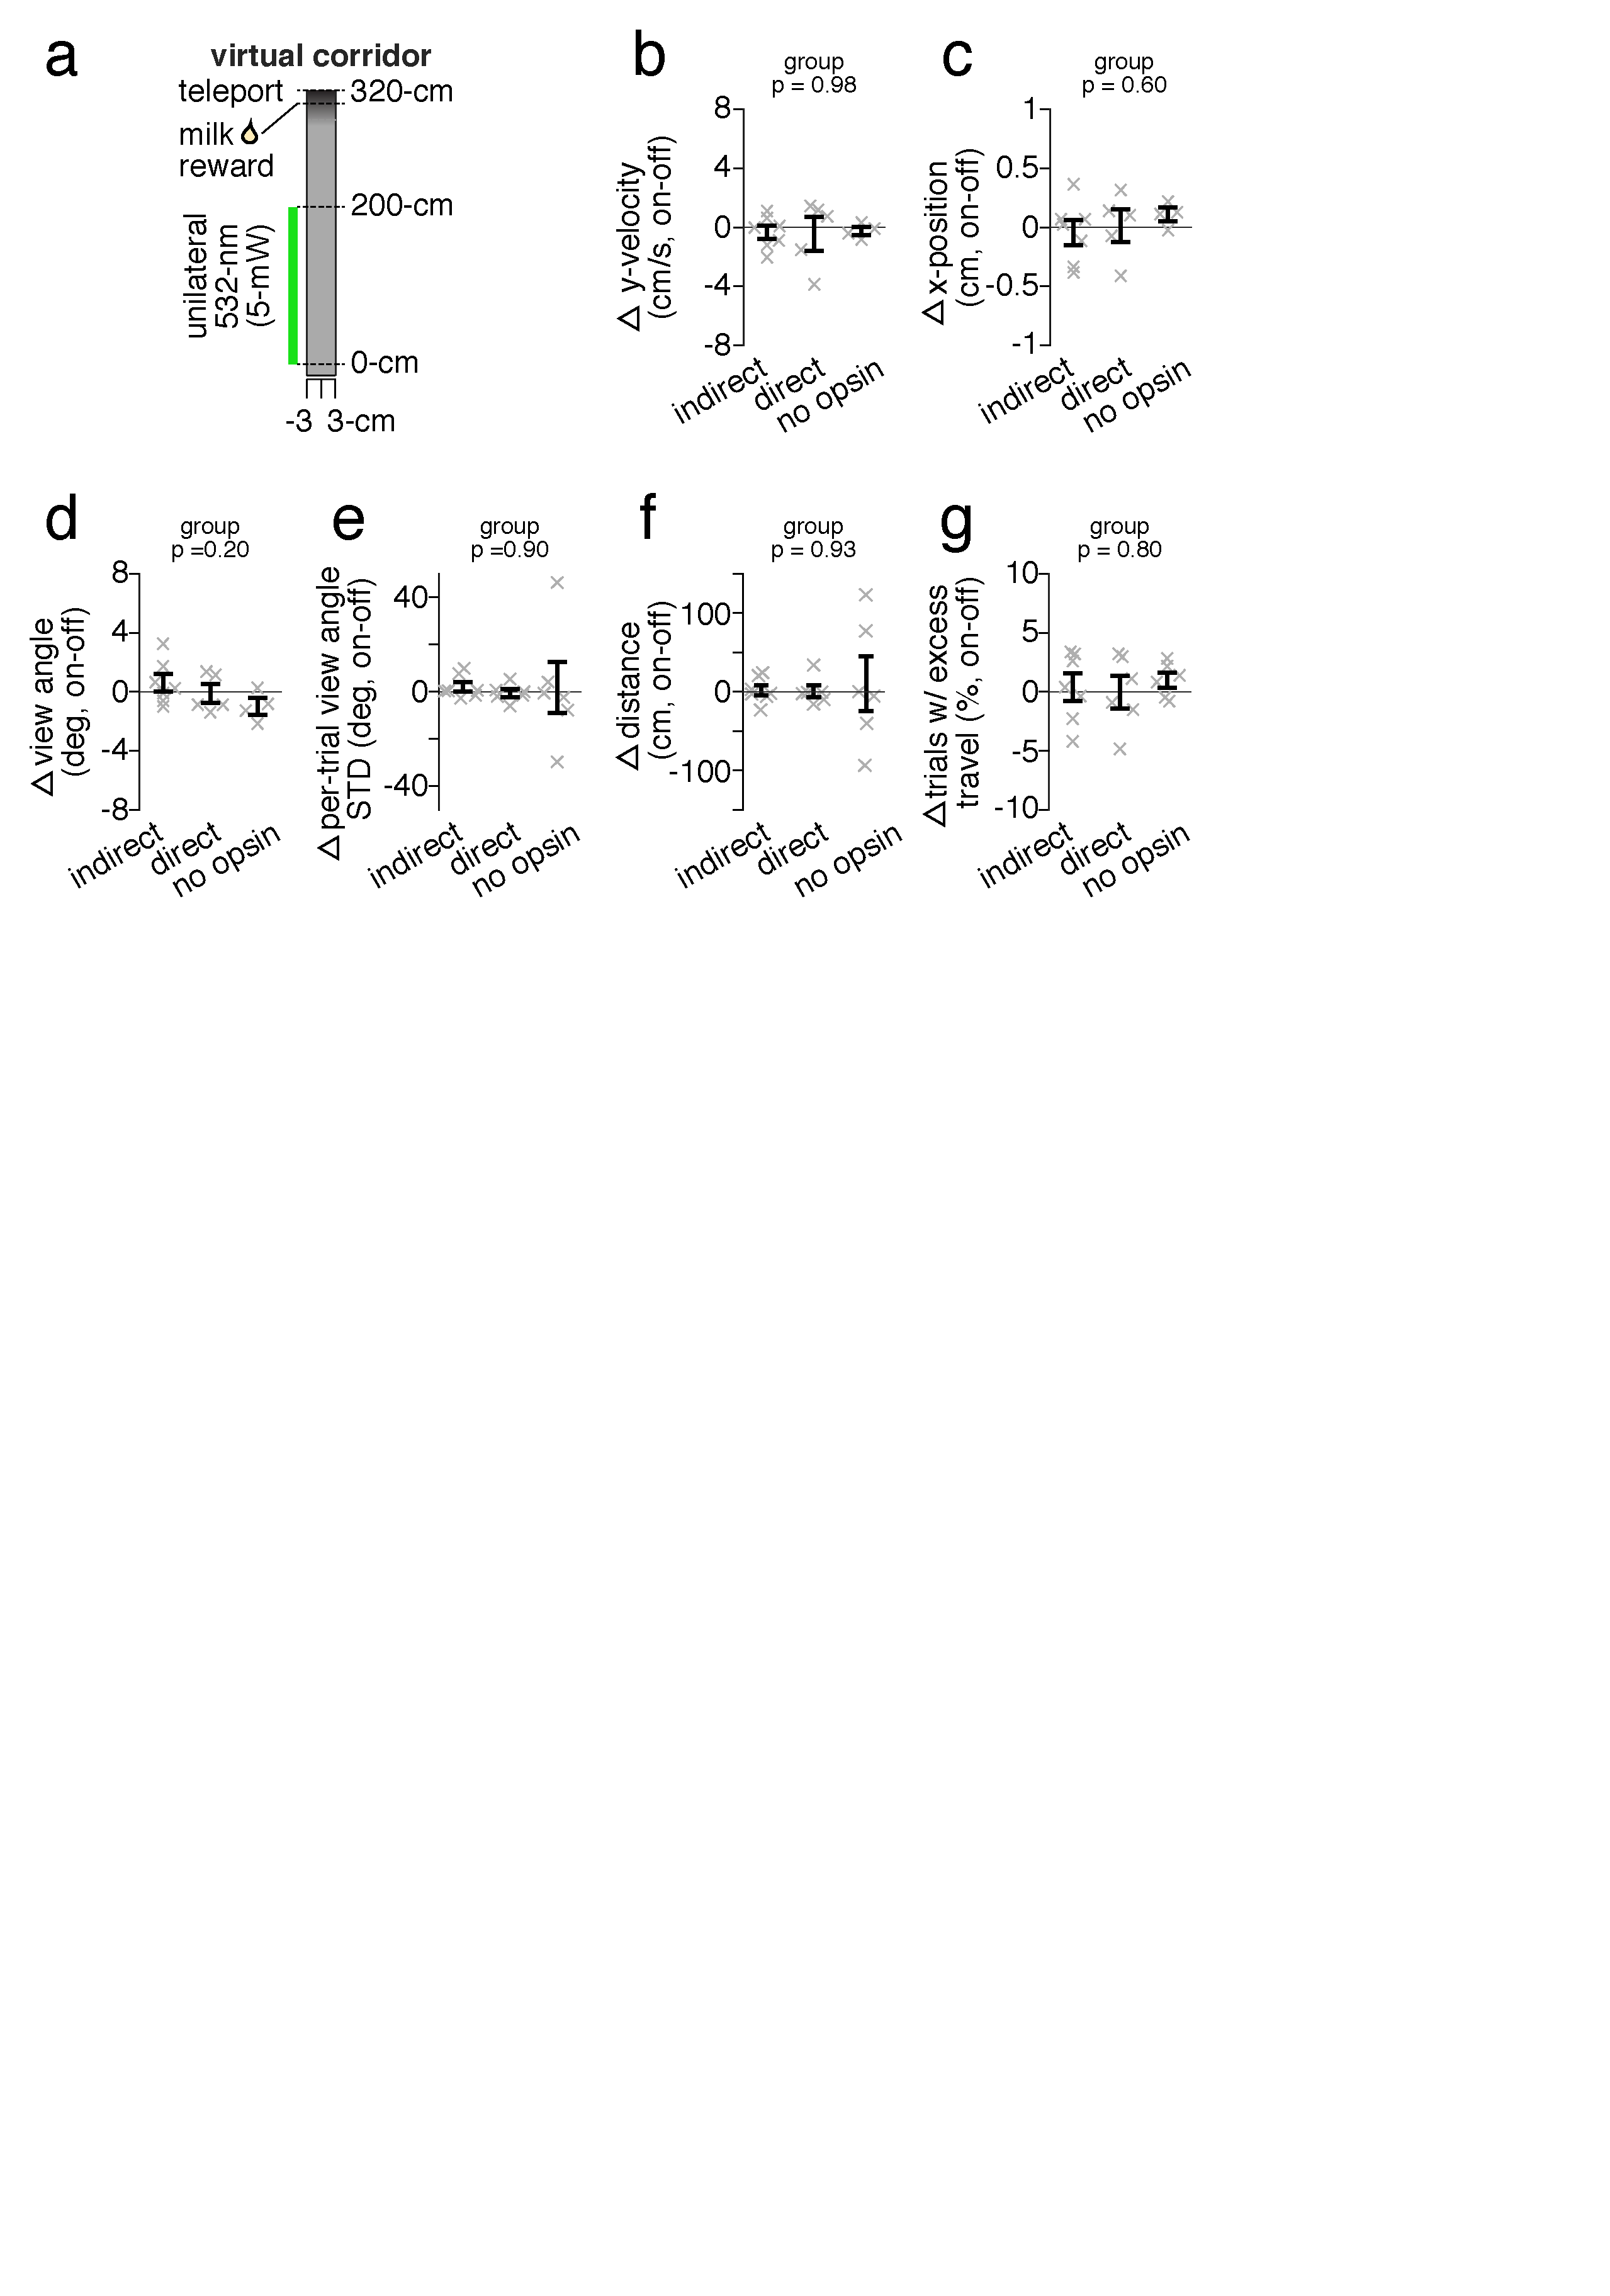
\includegraphics[width=0.90\linewidth]{ch7-appendix1/appendix1-figures/ExtData_Fig2.pdf}
    \caption[Non-significant motor effects of DMS pathway inhibition compared to non-opsin expressing controls during virtual corridor navigation]{\textbf{Non-significant motor effects of DMS pathway inhibition compared to non-opsin expressing controls during virtual corridor navigation.} (a) Schematic of virtual corridor and unilateral delivery of 532-nm light (5-mW) restricted to 0-200cm. (b) Difference in average y-velocity (cm/s) during laser on and off trials (on-off) for mice receiving indirect (n = 7 mice, n = 1,712 laser off and n = 1,288 laser on trials) or direct (n = 6 mice, n = 1,088 laser off and n = 757 laser on trials) pathway inhibition of the DMS, or DMS illumination alone (no opsin; n = 5 mice, n = 1,178 laser off and n = 827 laser on trials). p-value denotes significance of one-way ANOVA of group on delta y-velocity (p = 0.98, F2,13 = 0.02). }
    \label{fig:ap1:ext2}
  \end{center}
  \vspace{-1.5cm}
\end{figure}
\begin{figure}[t!]
%\vspace{-3cm}
  \contcaption{(c) Same as b but for difference in x-position (cm, on-off) contralateral to the laser hemisphere (p = 0.60, F2,13 = 0.53). (d) Same as c but for difference in view angle (deg, on-off) contralateral to the laser hemisphere (p = 0.20, F2,13 = 1.90). (e) Same as c but for difference in mean standard deviation in view angle (deg, on-off). The mean of the standard deviation in view angles sampled in 5-cm steps from 0-300 cm were calculated per trial, and then averaged across all laser off (or on) trials for a mouse (p = 0.94, F2,16 = 0.06). Indirect: n = 7 mice, n = 2,109 laser off and n = 1,574 laser on trials; direct: n = 6 mice, n = 1,330 laser off and n = 930 laser on trials; no opsin: n = 6  mice, n = 1,688 laser off and n = 1,199 laser on trials). (f) As in e but for difference in total distance travelled (cm, on-off) to complete a trial (p = 0.93, F2,16 = 0.08). (g) As in e but for the difference in percentage of trials with excess travel (defined as $>$10\% of corridor length to reward, or $>$330cm) (p = 0.76, F2,18 = 0.28). Throughout solid black lines indicate mean $\pm$ S.E.M. across mice and transparent ‘x’ denote individual mouse mean throughout.}% Continued caption
\end{figure}
\begin{figure}[t!]
%\vspace{-2.5cm}
  \begin{center}
    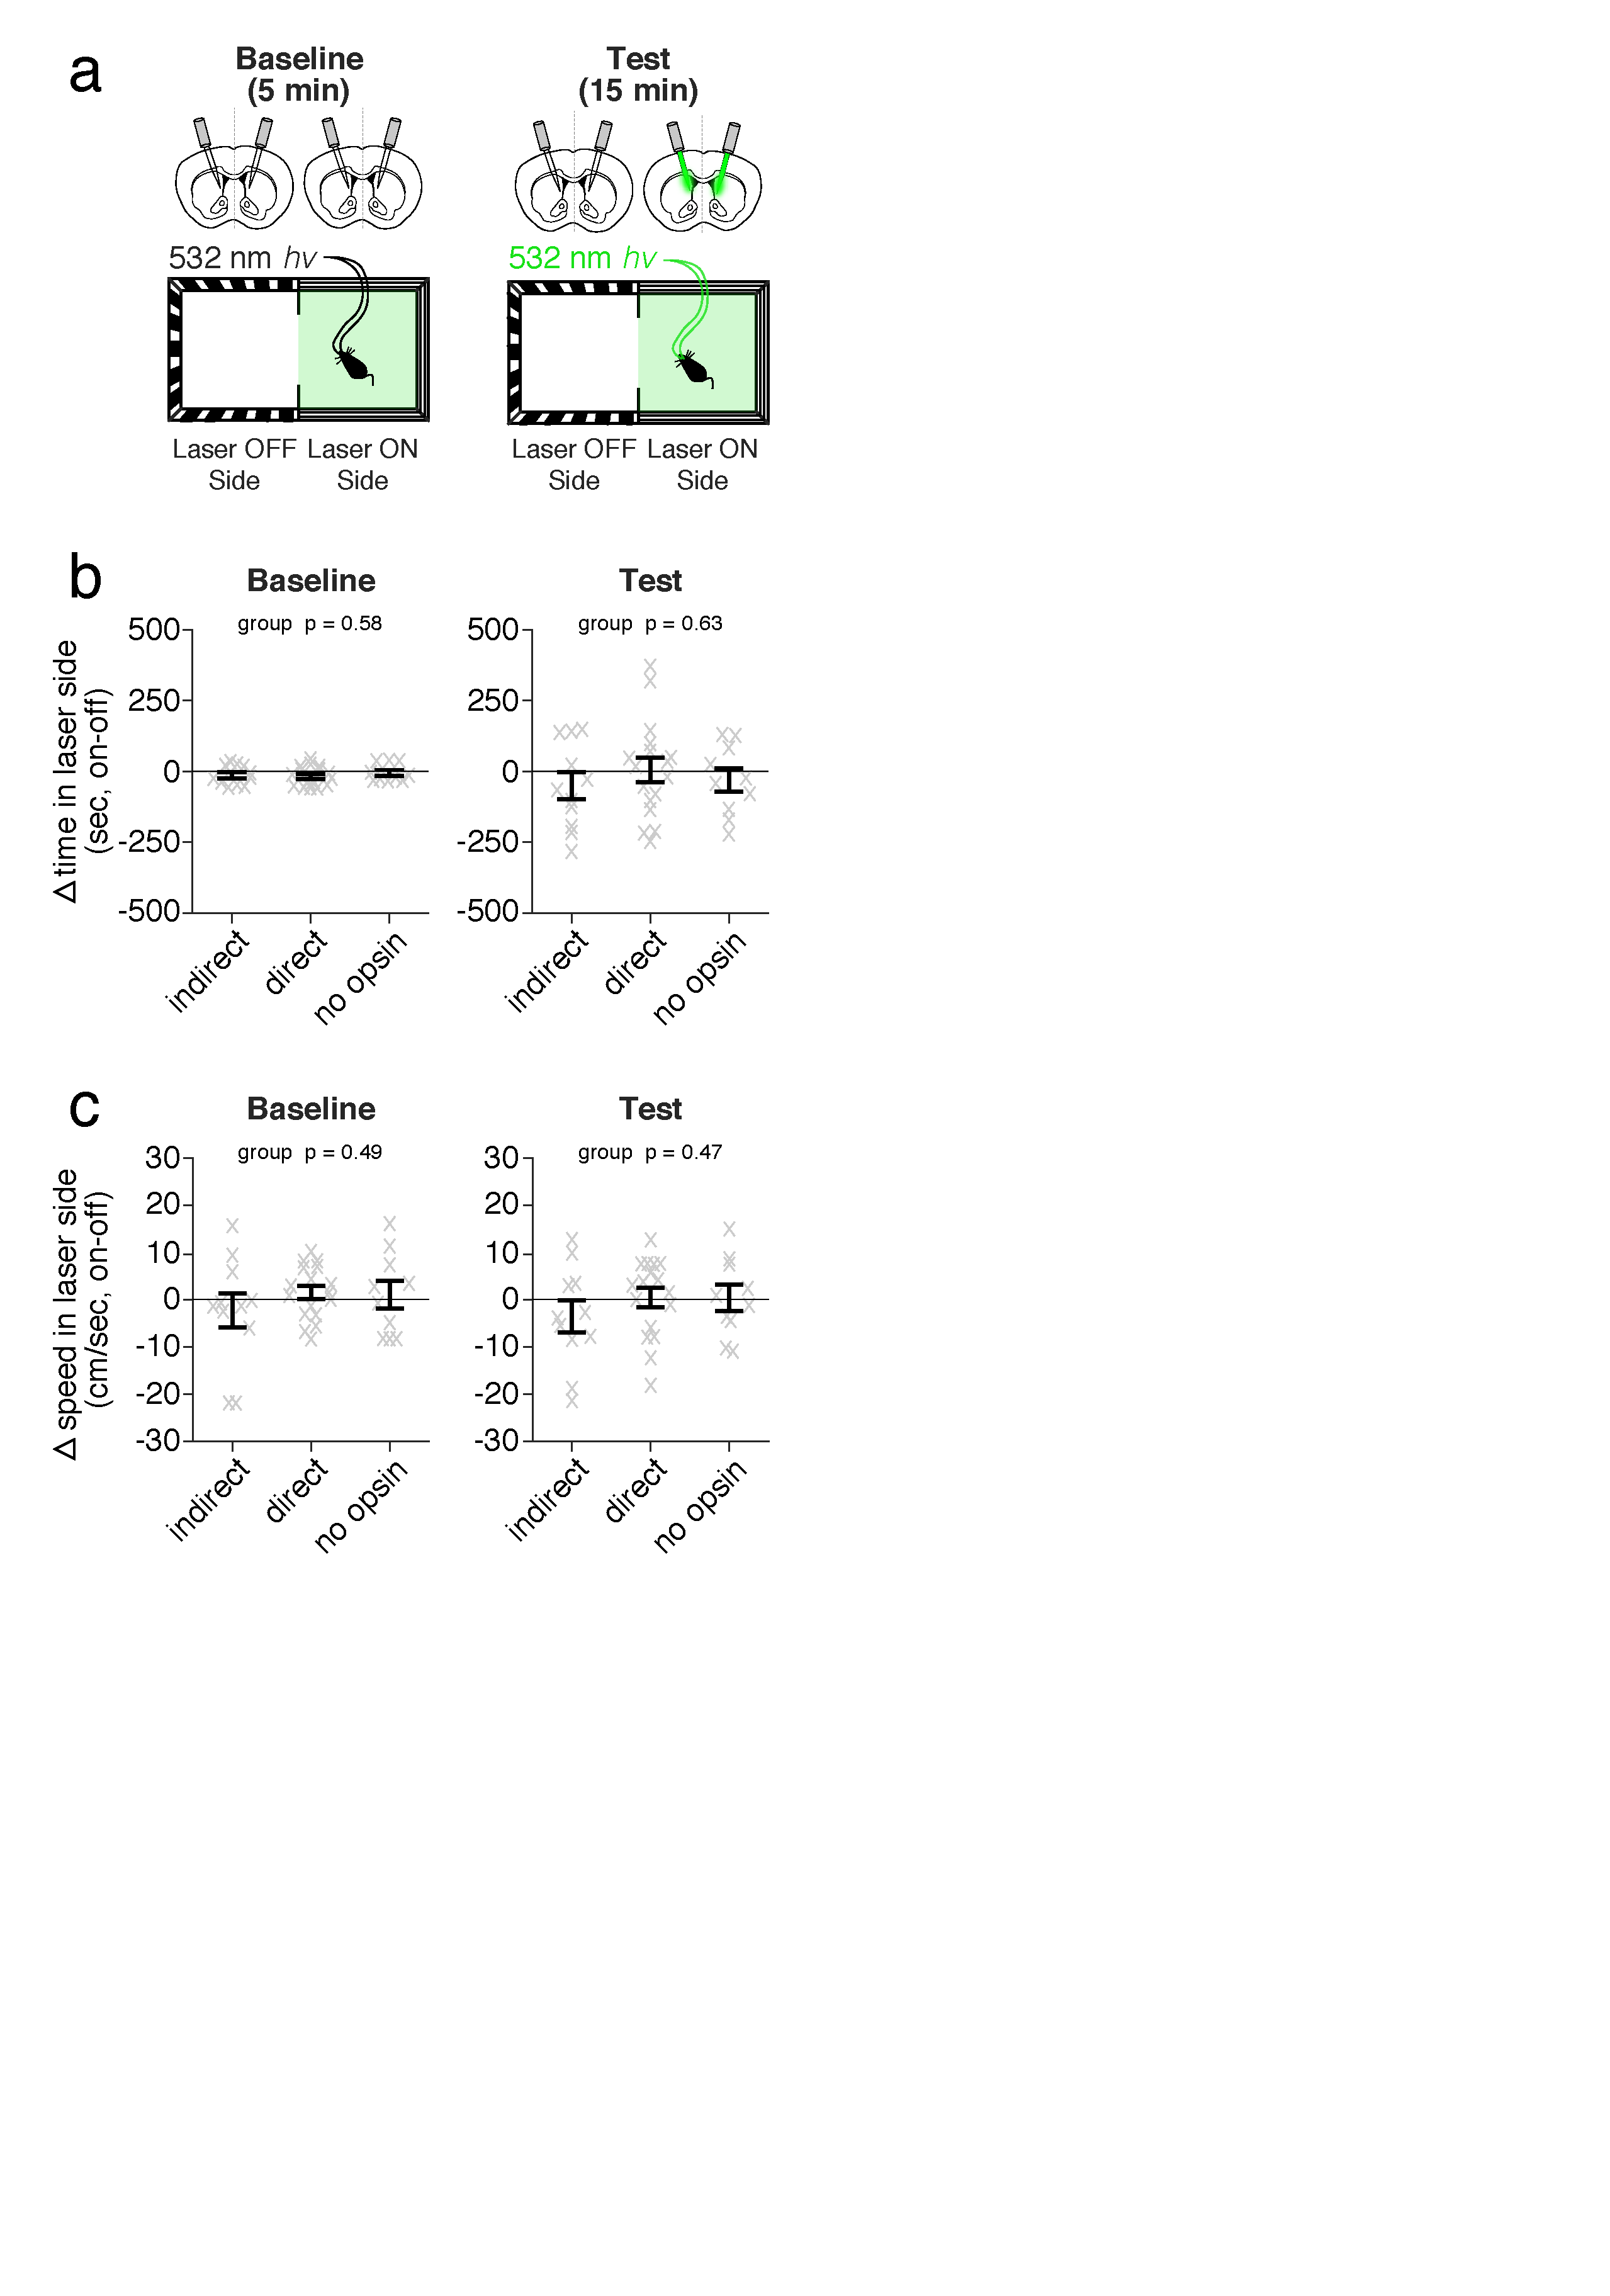
\includegraphics[width=0.47\linewidth]{ch7-appendix1/appendix1-figures/Supplementary_Fig3.pdf}
    \caption[No detectable effect of indirect or direct pathway inhibition on spatial preference and speed during a real-time conditioned place preference test]{\textbf{No detectable effect of indirect or direct pathway inhibition on spatial preference and speed during a real-time conditioned place preference test.} (a) Schematic of real-time conditioned place preference chamber and bilateral 532-nm laser illumination (5-mW) of the DMS. Left and right sub-chambers of equal size but with repeating vertical or horizontal black-and-white bar patterning distinguished each side, respectively. Mice underwent a 5-min preference test (left, Baseline) without any laser illumination, followed by a 20-min preference test (right, Test) in which mice received bilateral laser illumination only when occupying one of the two chamber sides (counterbalanced across mice). No illumination (Laser OFF) and illumination (Laser ON) sides during Baseline were defined based on the subsequent Test illumination side. (b) Delta time spent in chamber side (laser OFF - laser ON) during 5-min Baseline (left) and 20-min Test (right) for mice receiving DMS indirect (n = 9 mice) or direct (n = 20 mice) pathway inhibition, or DMS illumination alone (no opsin, n = 9 mice). Error bars denote mean and s.e.m. Grey transparent ‘x’ indicates individual mice. p-value denotes one-way ANOVA of group on delta time in the chamber side during Baseline (left: p = 0.73, F2,27 = 0.31) or Test (right: p = 0.10, F2,27 = 2.55).}
    \label{fig:ap1:supp3}
  \end{center}
  %\vspace{-1.5cm}
\end{figure}
\begin{figure}[t!]
%\vspace{-3cm}
  \contcaption{ (c) Average speed when mice occupied laser off (black) or laser on (green) chamber sides during Baseline (left) or Test (right) for same groups and order as in b. Solid bars indicate mean and s.e.m. Transparent grey lines indicate individual mouse mean. p-value denotes interaction of two-factor (between-subject: group, within-subject: laser) repeated measure ANOVA on speed during Baseline (left: group x laser interaction: p = 0.16, F1,35 = 2.07; laser: p = 0.28, F1,35 = 1.20) or Test (right: group x laser interaction: p = 0.07, F1,35 = 3.6; laser: p = 0.10, F1,35 = 2.8).}% Continued caption
\end{figure}
\begin{figure}[t!]
%\vspace{-2.5cm}
  \begin{center}
    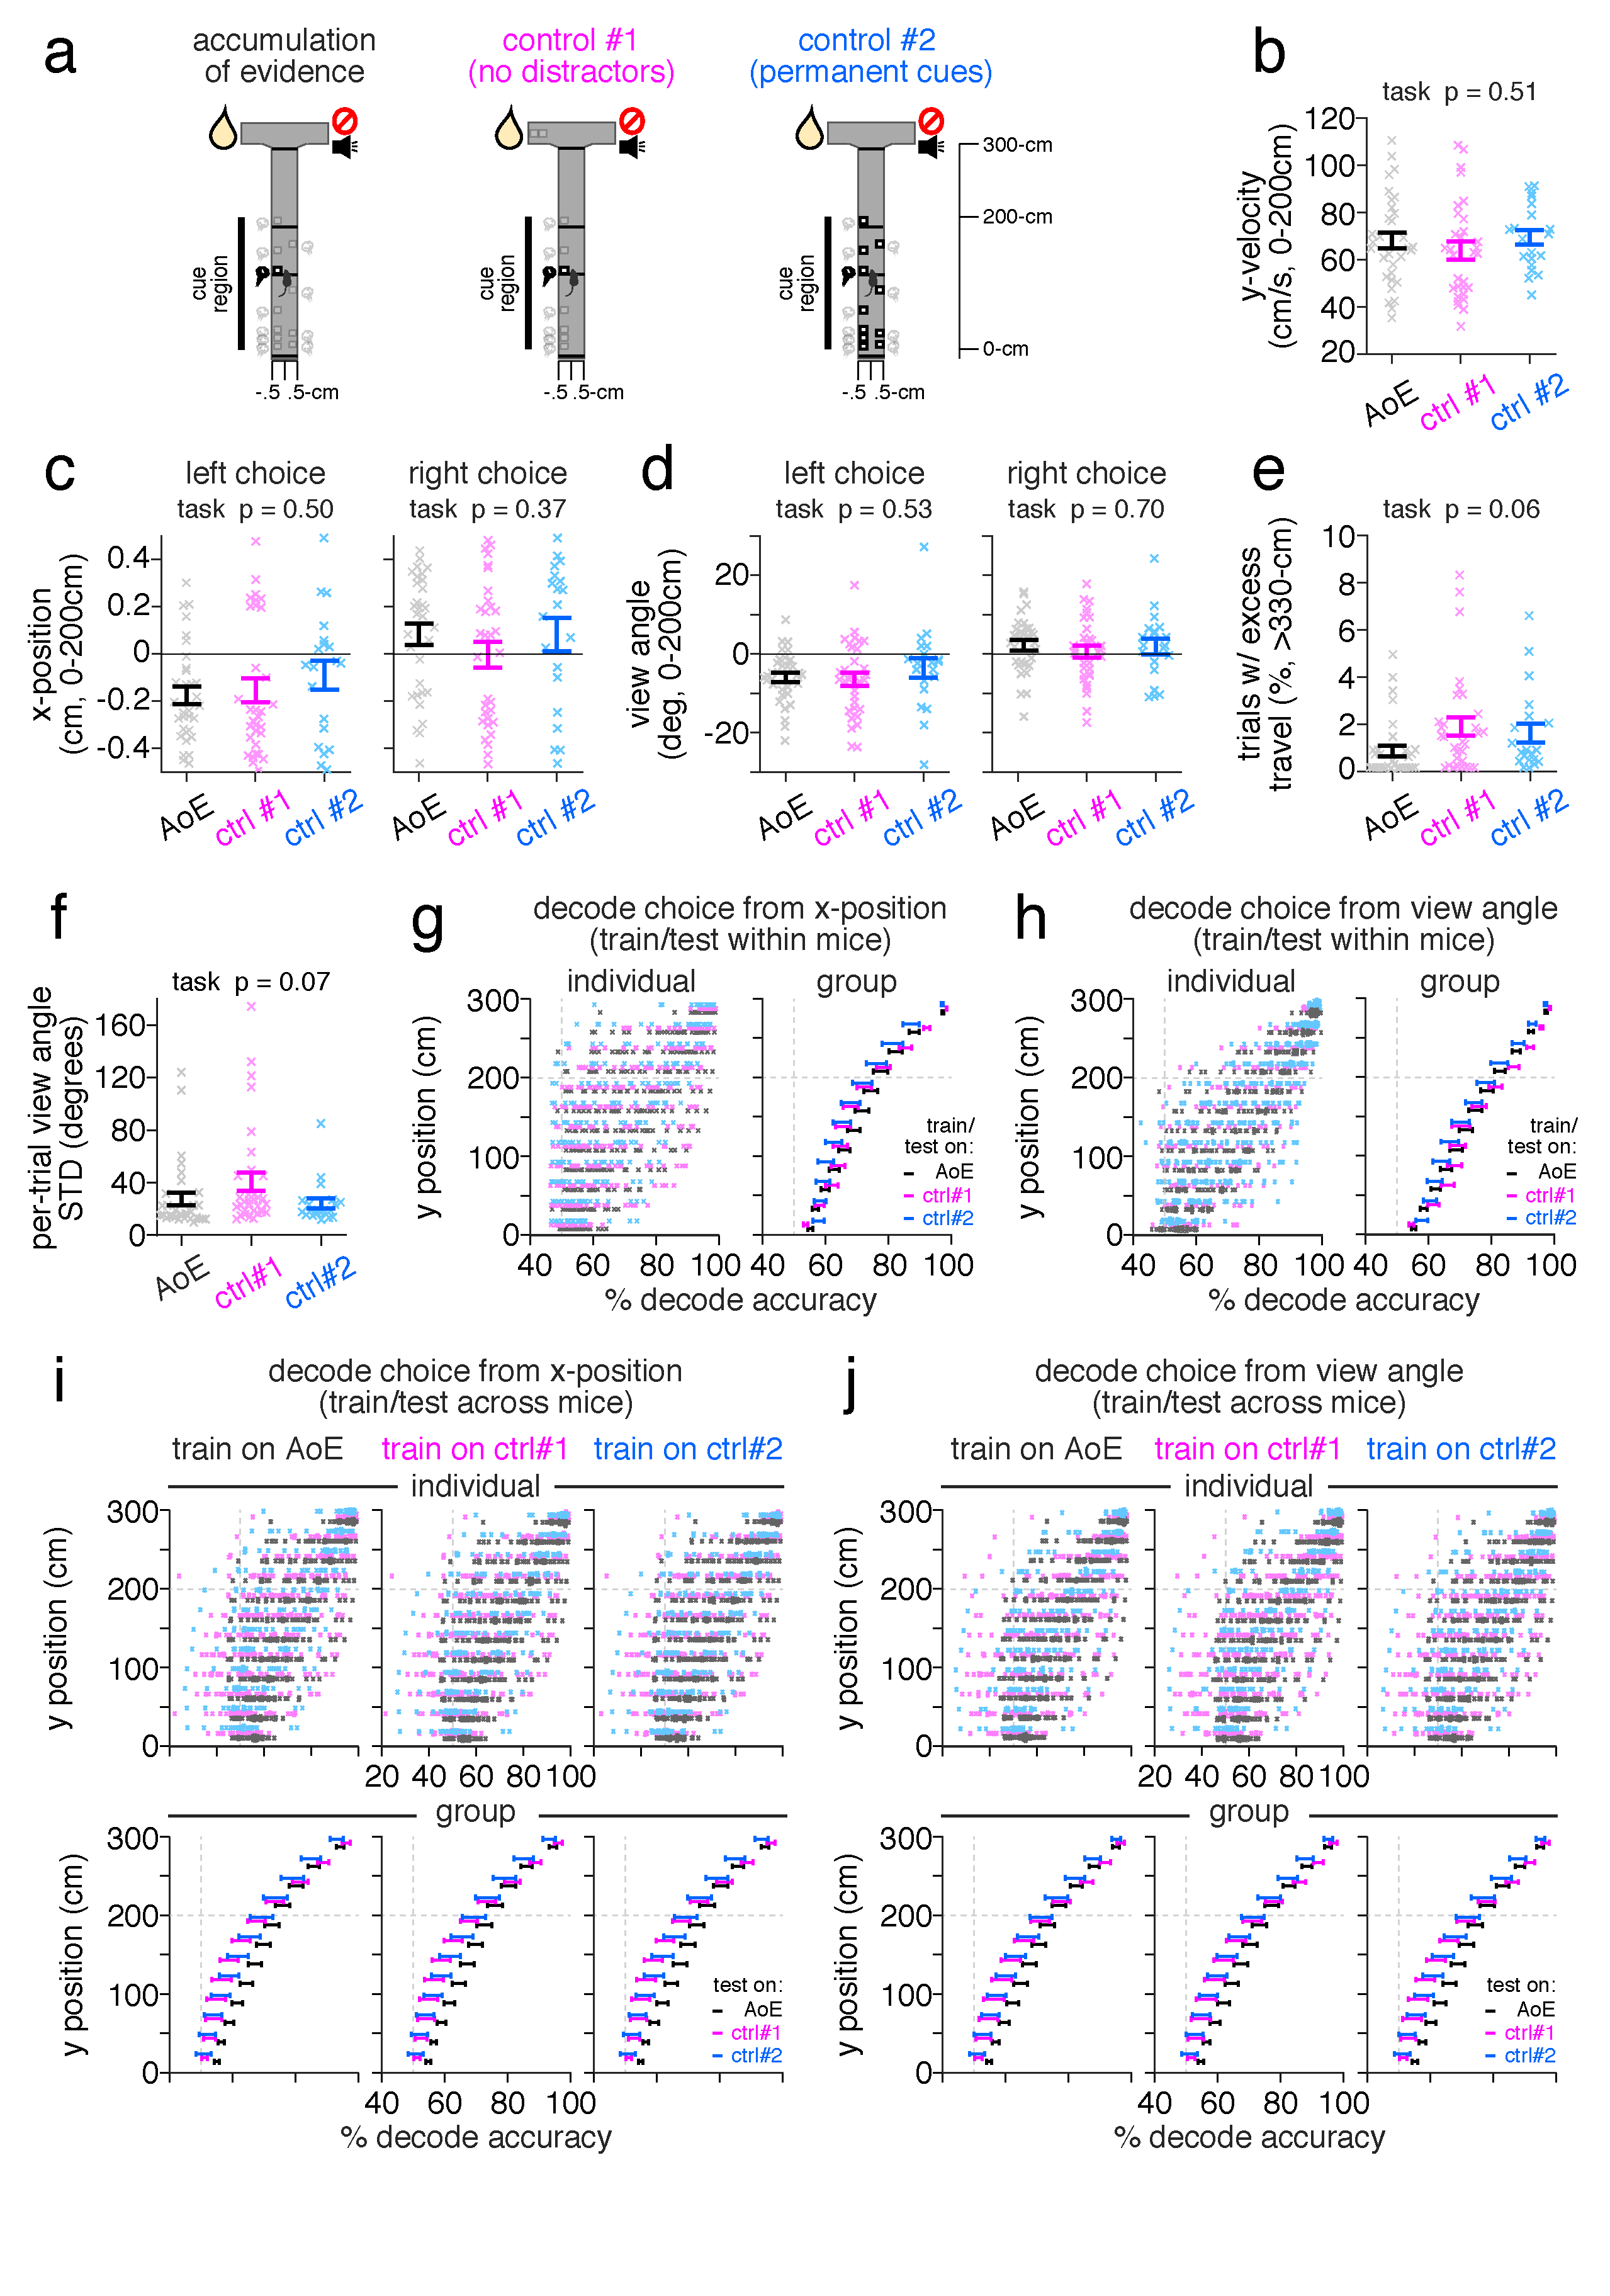
\includegraphics[width=0.90\linewidth]{ch7-appendix1/appendix1-figures/ExtData_Fig3.pdf}
    \caption[Similar motor performance across three virtual reality T-mazes]{\textbf{Similar motor performance across three virtual reality T-mazes.} }
    \label{fig:ap1:ext3}
  \end{center}
  %\vspace{-1.5cm}
\end{figure}
\begin{figure}[t!]
%\vspace{-3cm}
  \contcaption{ (a) Schematic of three virtual reality (VR)-based T-mazes that differ in task requirements. (b) Average y-velocity (cm/s) of mice during the cue region (0-200cm) of the accumulation of evidence task (black, n = 32 mice, n = 52,381 trials), no distractors (ctrl \#1) task (magenta: n = 32 mice, 56,783 trials), or permanent cues (ctrl \#2) task (cyan: n = 20 mice, n = 27,870 trials). Solid bars denote mean $\pm$ S.E.M. across mice while transparent ‘x’ denotes individual mouse mean. p-value denotes one-way ANOVA of task on y-velocity (p = 0.51, F2,80 = 0.67). (c) Same as b but for average x-position (cm) during the cue region (0-200cm) on left and right choice trials. p-value denotes one-way ANOVA of task on x-position (left choice: p = 0.50, F2,80 = 0.70; right choice: p = 0.37, F2,80 = 1.0). (d) Same as b but for average view angle (degrees) during the cue region (0-200cm) on left and right choice trials (left choice: p = 0.53, F2,80 = 0.64; right choice: p = 0.70, F2,80 = 0.37). (e) As in b but for average percent of trials with excess travel (defined as travel $>$10\% of maze stem, or $>$330cm). Accumulation of evidence: n = 32 mice, n = 53,833 trials; control \#2 (no distractors): n = 32 mice, n = 60,074 trials; control \#2 (permanent cues): n = 20 mice, n = 29,192 trials. p-value denotes one-way ANOVA of task on excess travel (p = 0.06, F2,81 = 2.9). (f) As in b but for mean standard deviation in view angle (degrees) per trial (n as in e). p-value denotes one-way ANOVA of task on view angle deviation (p = 0.07, F2,81 = 2.8). (g) Average accuracy of decoding left/right choice based on the trial-by-trial x-position (cm) of mice as a function of y-position in the maze (0-300cm in 25-cm bins). Training and test trial sets were selected within individual mice (80\% train, 5-fold cross-validation, re-sampled 10 times). Left: Each `x’ depicts decoding accuracy at each y-position bin for individual mice performing the evidence accumulation (black), no distractors (ctrl \#1, magenta), or permanent cues (ctrl \#2, cyan) tasks. Right: Group mean and $\pm$S.E.M. across mice for each task (n as in b). (h) Same as f but for average accuracy of decoding left/right choice based on the trial-by-trial view angle (degrees) of mice (n as in b). (i) Average accuracy of decoding left/right choice based on the trial-by-trial x-position (cm) of mice as a function of y-position in the maze (0-300cm in 25-cm bins). Training trial sets were randomly selected across all mice (50\% total trials, re-sampled 50 times) performing either the accumulation of evidence (left, AoE, black), no distractors (middle, ctrl \#1, magenta), or permanent cues (right, ctrl \#2, cyan) tasks. Testing trial sets were the 50\% of held-out trials in the task used for training, or all trials in the alternate tasks. Top: Each `x’ depicts average decoding accuracy across all training/tests sets at each y-position bin for individual mice performing the evidence accumulation (black), no distractors (ctrl \#1, magenta), or permanent cues (ctrl \#2, cyan) tasks. Right: Group mean and $\pm$S.E.M. across mice for each task (n as in a). (j) Same as I but for average accuracy of decoding left/right choice based on the trial-by-trial view angle (degrees) of mice (n as in b).}% Continued caption
\end{figure}
\begin{figure}[t!]
%\vspace{-2.5cm}
  \begin{center}
    \includegraphics[width=0.90\linewidth]{ch7-appendix1/appendix1-figures/ExtData_Fig4.pdf}
    \caption[Effects of pathway-specific DMS and NAc inhibition on psychometric performance across virtual reality tasks]{\textbf{Effects of pathway-specific DMS and NAc inhibition on psychometric performance across virtual reality tasks.} (a) Schematic of unilateral indirect pathway DMS inhibition with choice defined ipsilateral or contralateral to the hemisphere receiving 532-nm laser illumination. (b) Schematic of three virtual reality based decision-making tasks (left: accumulation of evidence; middle: control \#1, no distractors; right: control \#2, permanent cues) and laser illumination restricted to the cue region (0-200cm). (c) Percent of contralateral choice trials as a function of the difference in sensory cues (contralateral-ipsilateral) binned in increments of 5 from -15 to 15. Transparent lines indicate individual mouse mean during laser off (grey) and on (green) trials for mice receiving indirect-pathway DMS inhibition during the evidence accumulation (black, left), no distractors (magenta, ctrl \#1, middle), or permanent cues (cyan, ctrl \#2, right). Thick lines indicate mean $\pm$ S.E.M. across mice at each evidence bin during laser off (black) and on (green) trials. (d) Same as a but for mice receiving unilateral direct pathway DMS inhibition.  }
    \label{fig:ap1:ext4}
  \end{center}
  %\vspace{-1.5cm}
\end{figure}
\begin{figure}[t!]
%\vspace{-3cm}
  \contcaption{ (e) same as b. (f) Same as c but for mice receiving direct pathway DMS inhibition. (g) Same as a but for mice receiving unilateral DMS illumination in the absence of NpHR (no opsin). (h) Same as b. (i) same as c but for mice receiving unilateral DMS illumination in the absence of NpHR (no opsin). (j) Schematic of unilateral inhibition of NAc indirect (left) or  direct (middle) pathway, or NAc illumination in the absence of NpHR (no opsin). (k) Schematic of accumulation of evidence task and delivery of 532-nm light during the cue region (0-200cm). (l) As in c but for psychometric comparison between groups receiving NAc indirect or direct pathway inhibition, or NAc illumination in the absence of NpHR (no opsin). }% Continued caption
\end{figure}
\begin{figure}[t!]
%\vspace{-2.5cm}
  \begin{center}
    \includegraphics[width=0.75\linewidth]{ch7-appendix1/appendix1-figures/ExtData_Fig5.pdf}
    \caption[Effects of pathway-specific DMS inhibition on choice are larger in the most demanding task, and stronger than effects of pathway-specific NAc inhibition]{\textbf{Effects of pathway-specific DMS inhibition on choice are larger in the most demanding task, and stronger than effects of pathway-specific NAc inhibition.} (a) Schematic of three virtual reality based decision-making tasks (left: accumulation of evidence; middle: control \#1, no distractors; right: control \#2, permanent cues). (b) Schematic of unilateral }
    \label{fig:ap1:ext5}
  \end{center}
  %\vspace{-1.5cm}
\end{figure}
\begin{figure}[t!]
%\vspace{-3cm}
  \contcaption{ indirect pathway DMS inhibition with choice defined ipsilateral or contralateral to the hemisphere receiving 532-nm laser illumination (top). Difference in choice bias (\%, contralateral - ipsilateral) between laser on and off trials (on-off) in mice performing the accumulation of evidence (AoE, black), no distractors (ctrl \#1, magenta), or permanent cues (ctrl \#2, cyan) tasks. p-value denotes one-way ANOVA of task on delta (on-off) choice bias (p = 1.0 x 10-5, F2,22 = 20.2). Post-hoc comparisons reflect unpaired, two-tailed Wilcoxon ranksum tests on delta (on-off) choice bias (AoE, n = 11, vs ctrl \#1, n = 7: p = 8.0 x 10-4, z = 3.4; AoE vs ctrl \#2, n = 7: p = 0.001, z = 3.3). (c) Same as b but for direct pathway DMS inhibition. p-value denotes one-way ANOVA of task on delta (on-off) choice bias (p = 0.001, F2,23 = 9.4). Post-hoc comparisons reflect two-tailed, unpaired Wilcoxon ranksum tests (AoE, n = 10, vs ctrl \#1, n = 9: p = 0.002, z = -3.0; AoE vs ctrl \#2, n = 7: p = 0.005, z = -2.8). (d) Same as b but for DMS illumination in the absence of NpHR (no opsin). p-value denotes one-way ANOVA of task on delta (on-off) choice bias (p = 0.09, F2,16 = 2.8). Post-hoc comparisons reflect two-tailed, unpaired Wilcoxon ranksum tests (AoE, n= 11, vs ctrl \#1, n = 4: p = 0.65, z = 0.46; AoE vs ctrl \#2, n = 6: p = 0.06, z = 1.8). (e) Schema of evidence accumulation task (left), unilateral inhibition of indirect pathway in the DMS (middle left) or NAc (middle right), and delta (on-off) choice bias in mice receiving indirect pathway DMS (n = 11) or NAc (n = 9) inhibition (right). Statistical comparison reflects two-tailed, unpaired Wilcoxon ranksum test (DMS vs NAc: p = 2.6 x 10-4, z = 3.6). (f) Same as e but for direct pathway DMS (n = 10) or NAc (n = 10) inhibition. Statistical comparison reflects two-tailed, unpaired Wilcoxon ranksum test (DMS vs NAc: p = 1.8 x 10-4, z = -3.7). Throughout solid bars denote mean $\pm$ S.E.M. across mice and transparent ‘x’ denote individual mouse means. }% Continued caption
\end{figure}
\begin{figure}[t!]
%\vspace{-2.5cm}
  \begin{center}
    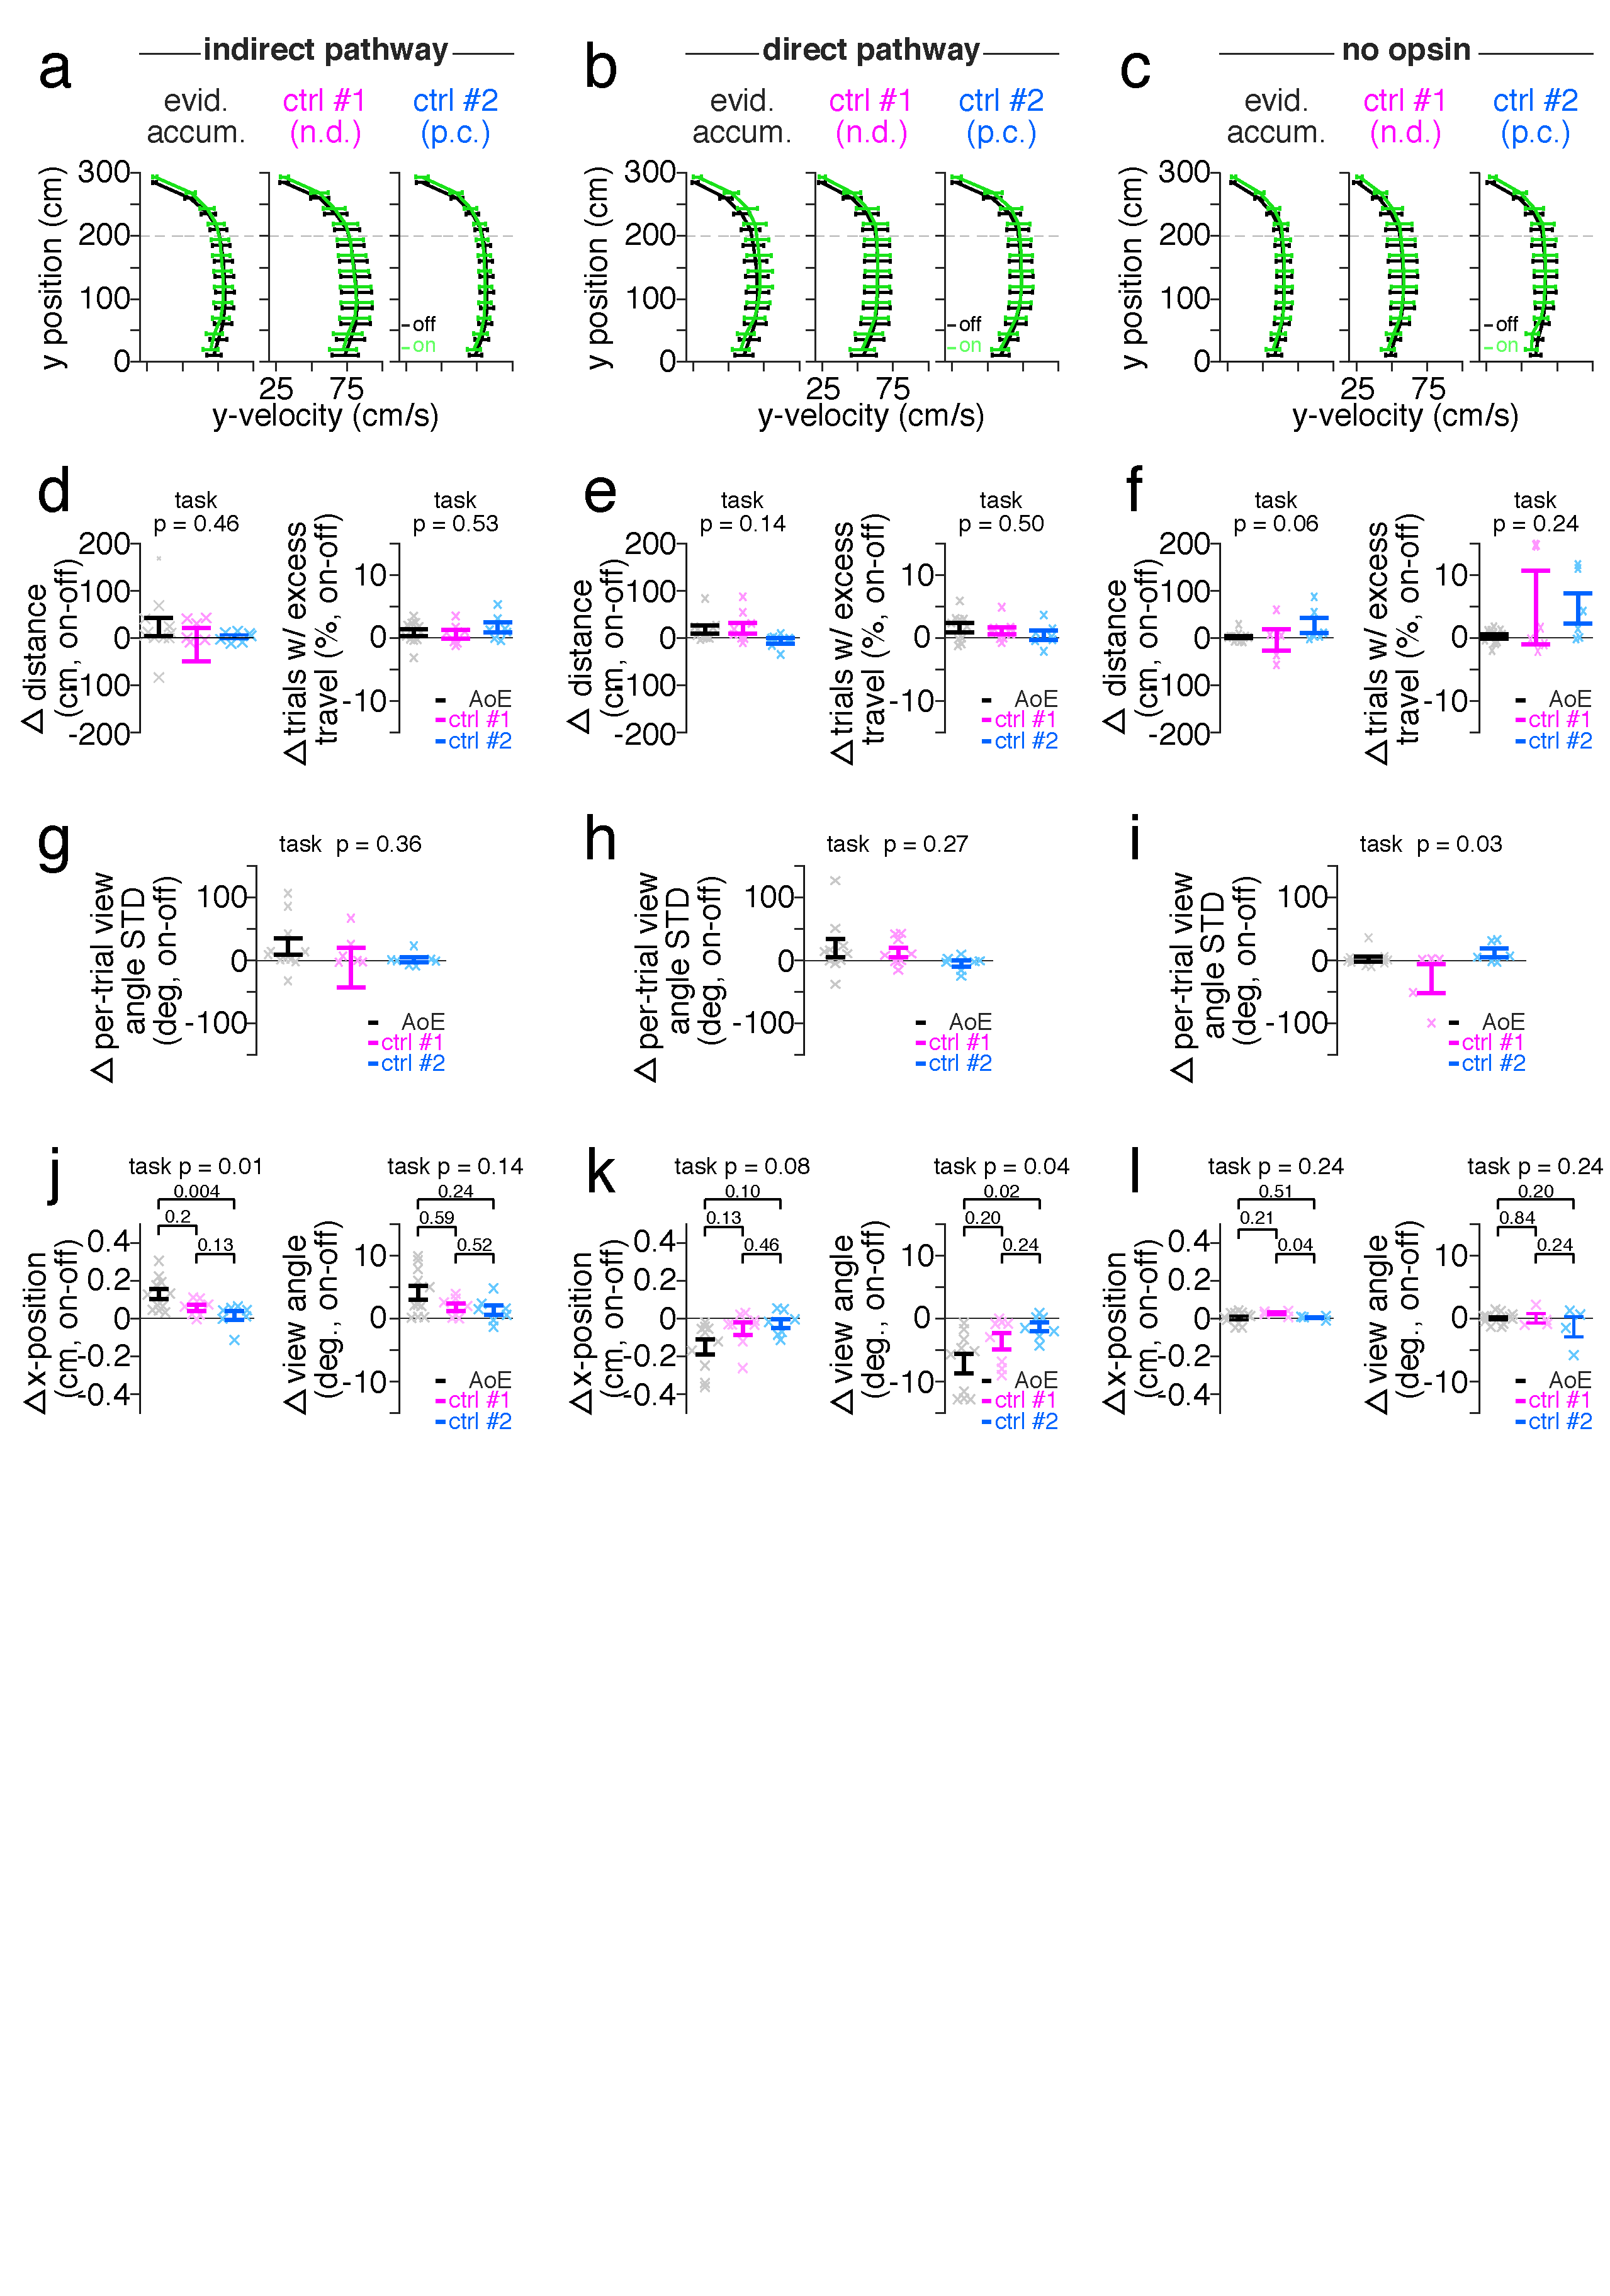
\includegraphics[width=0.90\linewidth]{ch7-appendix1/appendix1-figures/ExtData_Fig6.pdf}
    \caption[Inhibition of DMS pathways has limited impact on motor performance across VR-based decision-making tasks]{\textbf{Inhibition of DMS pathways has limited impact on motor performance across VR-based decision-making tasks.} (a) Mean $\pm$ S.E.M. y-velocity (cm/s) as a function of y-position (0- 300cm in 25cm bins) during laser off (black) or laser on (green) trials across mice receiving DMS indirect pathway inhibition during the evidence accumulation (left: n = 11 mice, n = 16,935 laser off and n = 3,390 laser on trials), no distractors (middle, ctrl \#1:  n = 7 mice, n = 13,706 laser off and n = 3,288 laser on trials) or permanent cues (right, ctrl \#2:  n = 6 mice, n = 4,033 laser off and n = 929 laser on trials). (b) Same as a but for mice receiving direct pathway inhibition during the evidence accumulation (left: n = 10 mice, n = 14,030 laser off and n = 3,103 laser on trials), no distractors (middle, ctrl \#2: n = 8 mice, n = 14,647 laser off and n = 3,682 laser on trials) or permanent cues (right, ctrl \#3:  n = 7 mice, n = 6,061 laser off and n = 1,494 laser on trials) tasks. (c) Same as a but for mice receiving DMS illumination in the absence of NpHR (no opsin) during the evidence accumulation (left: n = 11 mice, n = 21,422 laser off and n = 5,113 laser on trials), no distractors (middle, ctrl \#1:  n = 4 mice, n = 3,654 laser off and n = 901 laser on trials), or permanent cues (right, ctrl \#2:  n = 4 mice, n = 3,975 laser off and n = 923 laser on trials) tasks. (d) Mean $\pm$ S.E.M. in delta (on-off) distance (cm) traveled (left) and delta (on-off) trials (\%) with excess travel greater than 10\% of maze stem (or $>$330cm) (right) in mice receiving indirect pathway inhibition during the evidence accumulation (black, n = 11 mice, n = 22,090 laser off and n = 4,378 laser on trials), no distractors (magenta,  n = 7 mice, n = 14,826 }
    \label{fig:ap1:ext6}
  \end{center}
  %\vspace{-1.5cm}
\end{figure}
\begin{figure}[t!]
%\vspace{-3cm}
  \contcaption{ (e) Same as d but for delta (on-off) distance (cm) traveled (left) or delta percent trials with excess travel (right) in mice receiving direct pathway inhibition during the evidence accumulation (black, n = 10 mice, n = 20,914 laser off and n = 4,721 laser on trials), no distractors (magenta,  n = 9 mice, n = 15,778 laser off and n = 3,992 laser on trials), or permanent cues (n = 7 mice, n = 6,430 laser off and n = 1,591 laser on trials) tasks. p-value denotes one-way ANOVA of task on delta (on-off) distance (p = 0.13, F2,23 = 2.2) or excess travel (p = 0.50, F2,23 = 0.71). (f) Same as d but for delta (on-off) in distance (cm) traveled (left) or percent trials with excess travel (right) in mice receiving DMS illumination in the absence of NpHR (no opsin) during the evidence accumulation (black, n = 11 mice, n = 28,557 laser off and n = 6,772 laser on trials), no distractors (magenta,  n = 5 mice, n = 4,118 laser off and n = 1,002 laser on trials), or permanent cues (n = 6 mice, n = 4,360 laser off and n = 1,038 laser on trials) tasks. p-value denotes one-way ANOVA of task on delta (on-off) distance (p = 0.06, F2,19 = 3.3) or excess travel (p = 0.23, F2,19 = 1.6). (g) Same as d but for delta (on-off) in per-trial standard deviation in view angle in mice receiving DMS indirect pathway inhibition across tasks (p = 0.34, F2,22 = 1.1, n as in d). (h) Same as g but for mice receiving DMS direct pathway inhibition across tasks (p = 0.27, F2,23 = 1.4, n as in e). (i) Same as g but for mice receiving DMS illumination (no opsin) in the absence of NpHR (p = 0.03, F2,19 = 4.3, n as in f). (j) Delta (on-off) x-position (cm) (left) or view angle (degrees) (right) during the cue region (0-200 cm) in mice receiving DMS indirect pathway inhibition during the accumulation of evidence (black), no distractors (control \#1, magenta), or permanent cues (control \#2, cyan) tasks (n as in a). One-way ANOVA of task on delta (on-off) x-position (p = 0.01, F2,22 = 5.6). Post-hoc, two-tailed, unpaired Wilcoxon ranksum test on delta (on-off) x-position (AoE v control \#1: p = 0.2, z = 1.3; AoE v control \#2: p = 0.004, z = 2.9; control \#1 v control \#2: p = 0.13, z = 1.5). One-way ANOVA of task on delta (on-off) view angle (p = 0.14, F2,22 = 2.2). Post-hoc, two-tailed, unpaired Wilcoxon ranksum test on delta (on-off) view angle (AoE v control \#1: p = 0.58, z = 0.5; AoE v control \#2: p = 0.24, z = 1.78; control \#1 v control \#2: p = 0.52, z = 0.6). (k) Same as j but for mice receiving DMS direct pathway inhibition (n as in b). One-way ANOVA of task on delta (on-off) x-position (p = 0.08, F2,23 = 2.8). Post-hoc, two-tailed unpaired Wilcoxon ranksum test on delta (on-off) x-position (AoE v control \#1: p = 0.13, z = -1.5; AoE v control \#2: p = 0.1, z = -1.6; control \#1 v control \#2: p = 0.46, z = -0.7). One-way ANOVA of task on delta (on-off) view angle (p = 0.02, F2,23 = 3.6). Post-hoc, two-tailed, unpaired Wilcoxon ranksum test on delta (on-off) view angle (AoE v control \#1: p = 0.21, z = -1.3; AoE v control \#2: p = 0.03, z = -2.1; control \#1 v control \#2: p = 0.24, z = -1.6). (l) Same as j but for mice receiving DMS illumination in the absence of NpHR (no opsin, n as in c). One-way ANOVA of task on delta (on-off) x-position (p = 0.24, F2,18 = 1.54). Post-hoc, two-tailed, unpaired Wilcoxon ranksum test on delta (on-off) x-position (AoE v control \#1: p = 0.21, z = -1.24; AoE v control \#2: p = 0.51, z = 0.06; control \#1 v control \#2: p = 0.04, z = 2.0). One-way ANOVA of task on delta (on-off) view angle (p = 0.23, F2,18 = 1.56). Post-hoc, two-tailed, unpaired Wilcoxon ranksum test on delta (on-off) view angle (AoE v control \#1: p = 0.84, z = 0.19; AoE v control \#2: p = 0.20, z = 1.2; control \#1 v control \#2: p = 0.24, z = 1.7). Throughout solid bars denote mean $\pm$ S.E.M. and transparent ‘x’ indicates individual mouse mean.}% Continued caption
\end{figure}
\begin{figure}[t!]
%\vspace{-2.5cm}
  \begin{center}
    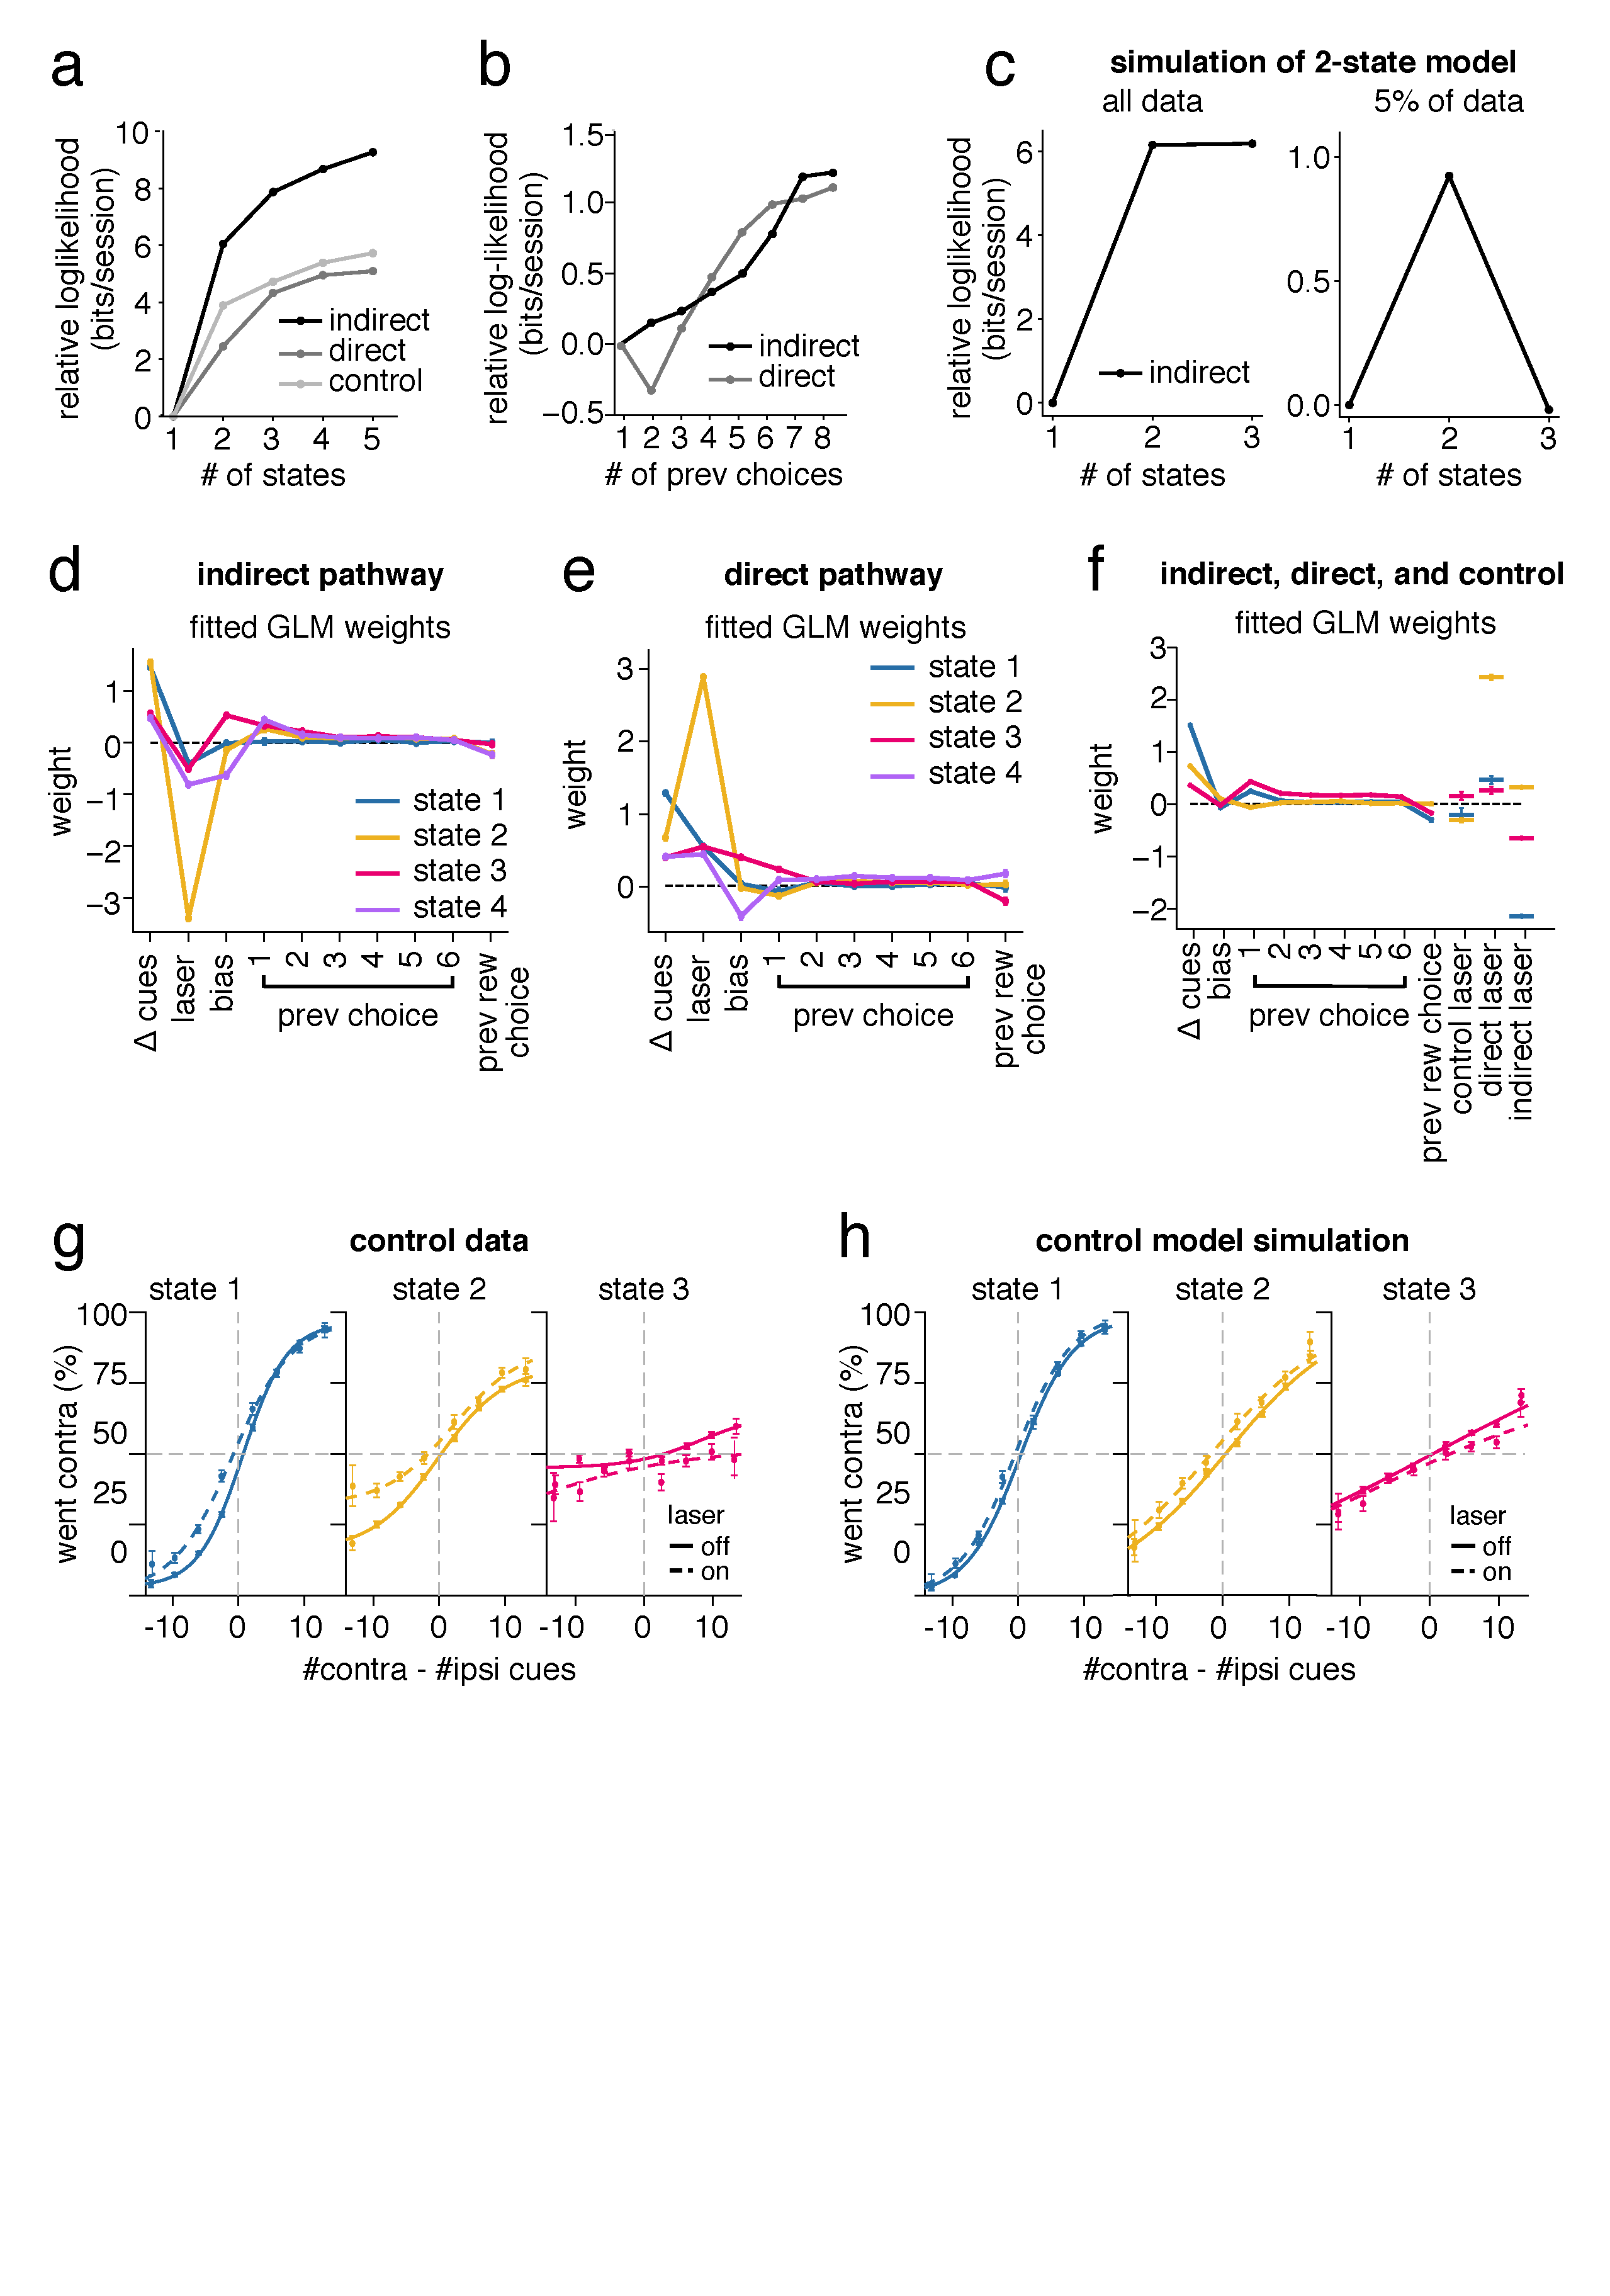
\includegraphics[width=0.90\linewidth]{ch7-appendix1/appendix1-figures/ExtData_Fig7.pdf}
    \caption[Model selection and control data analyses for the GLM-HMM]{\textbf{Model selection and control data analyses for the GLM-HMM.} (a) Comparison of the log-likelihood of the data using GLM-HMMs with different numbers of states for mice inhibited in the DMS direct pathway (dark gray), or indirect pathway (light gray), and mice without DMS opsin (black). All values are relative to the log-likelihood of the standard GLM (1-state GLM-HMM). Values are calculated in bits per session (see Methods). Solid curves denote mean $\pm$ S.E.M. of five different test sets. Held-out data for test sets was selected as a random 20\% of sessions, using the same number of sessions for each mouse. (b) Same as a but with different numbers of previous choice covariates using a 3-state GLM-HMM. (c) Comparison of the log-likelihood of simulated data using GLM-HMMs with different numbers of states. Data was simulated from a 2-state GLM-HMM that had been fit to data for mice inhibited in the indirect pathway of the DMS and then cross-validation performed either on the entire simulated dataset (~54000 trials, left) or a subset of 5\% of the data (2600 trials, right). All values are relative to the log-likelihood of the 1-}
    \label{fig:ap1:ext7}
  \end{center}
  %\vspace{-1.5cm}
\end{figure}
\begin{figure}[t!]
%\vspace{-3cm}
  \contcaption{state GLM. Values are calculated in bits per session (see Methods). Solid curves denote the average of five different test sets. Held-out data for test sets was selected as a random 20\% of sessions. (d) Fitted GLM weights for the 4-state model using aggregated data from all mice inhibited in the indirect pathway of the DMS. Error bars denote ($\pm$1) posterior standard deviation for each weight. The magnitude of the weight represents the relative importance of that covariate in predicting choice, whereas the sign of the weight indicates the side bias. (e) Same as d but for mice inhibited in the DMS direct pathway. (f) GLM weights fitted to a concatenated data set consisting of the indirect, direct, and control (no opsin) groups. Solid lines on the left connect covariates that are shared across groups. Horizontal marks on the right denote laser weights, which were learned separately for each group. Error bars denote the posterior standard deviation of each weight. (g) Percent of contralateral choice based on the difference in contralateral versus ipsilateral cues in each trial for mice in the control (no opsin) group. To compute psychometric functions, trials were assigned to each state by taking the maximum of the model’s posterior state probabilities on each trial. Error bars denote $\pm$1 S.E.M. for light off (solid) and light on (dotted) trials. Solid curves denote logistic fits to the concatenated data across mice for light off (solid) and light on (dotted) trials. (h) Same as f but for data simulated from the model fit to mice in the control group  (see \ref{sec:appendix1:methods}).}% Continued caption
\end{figure}
\begin{figure}[t!]
%\vspace{-2.5cm}
  \begin{center}
    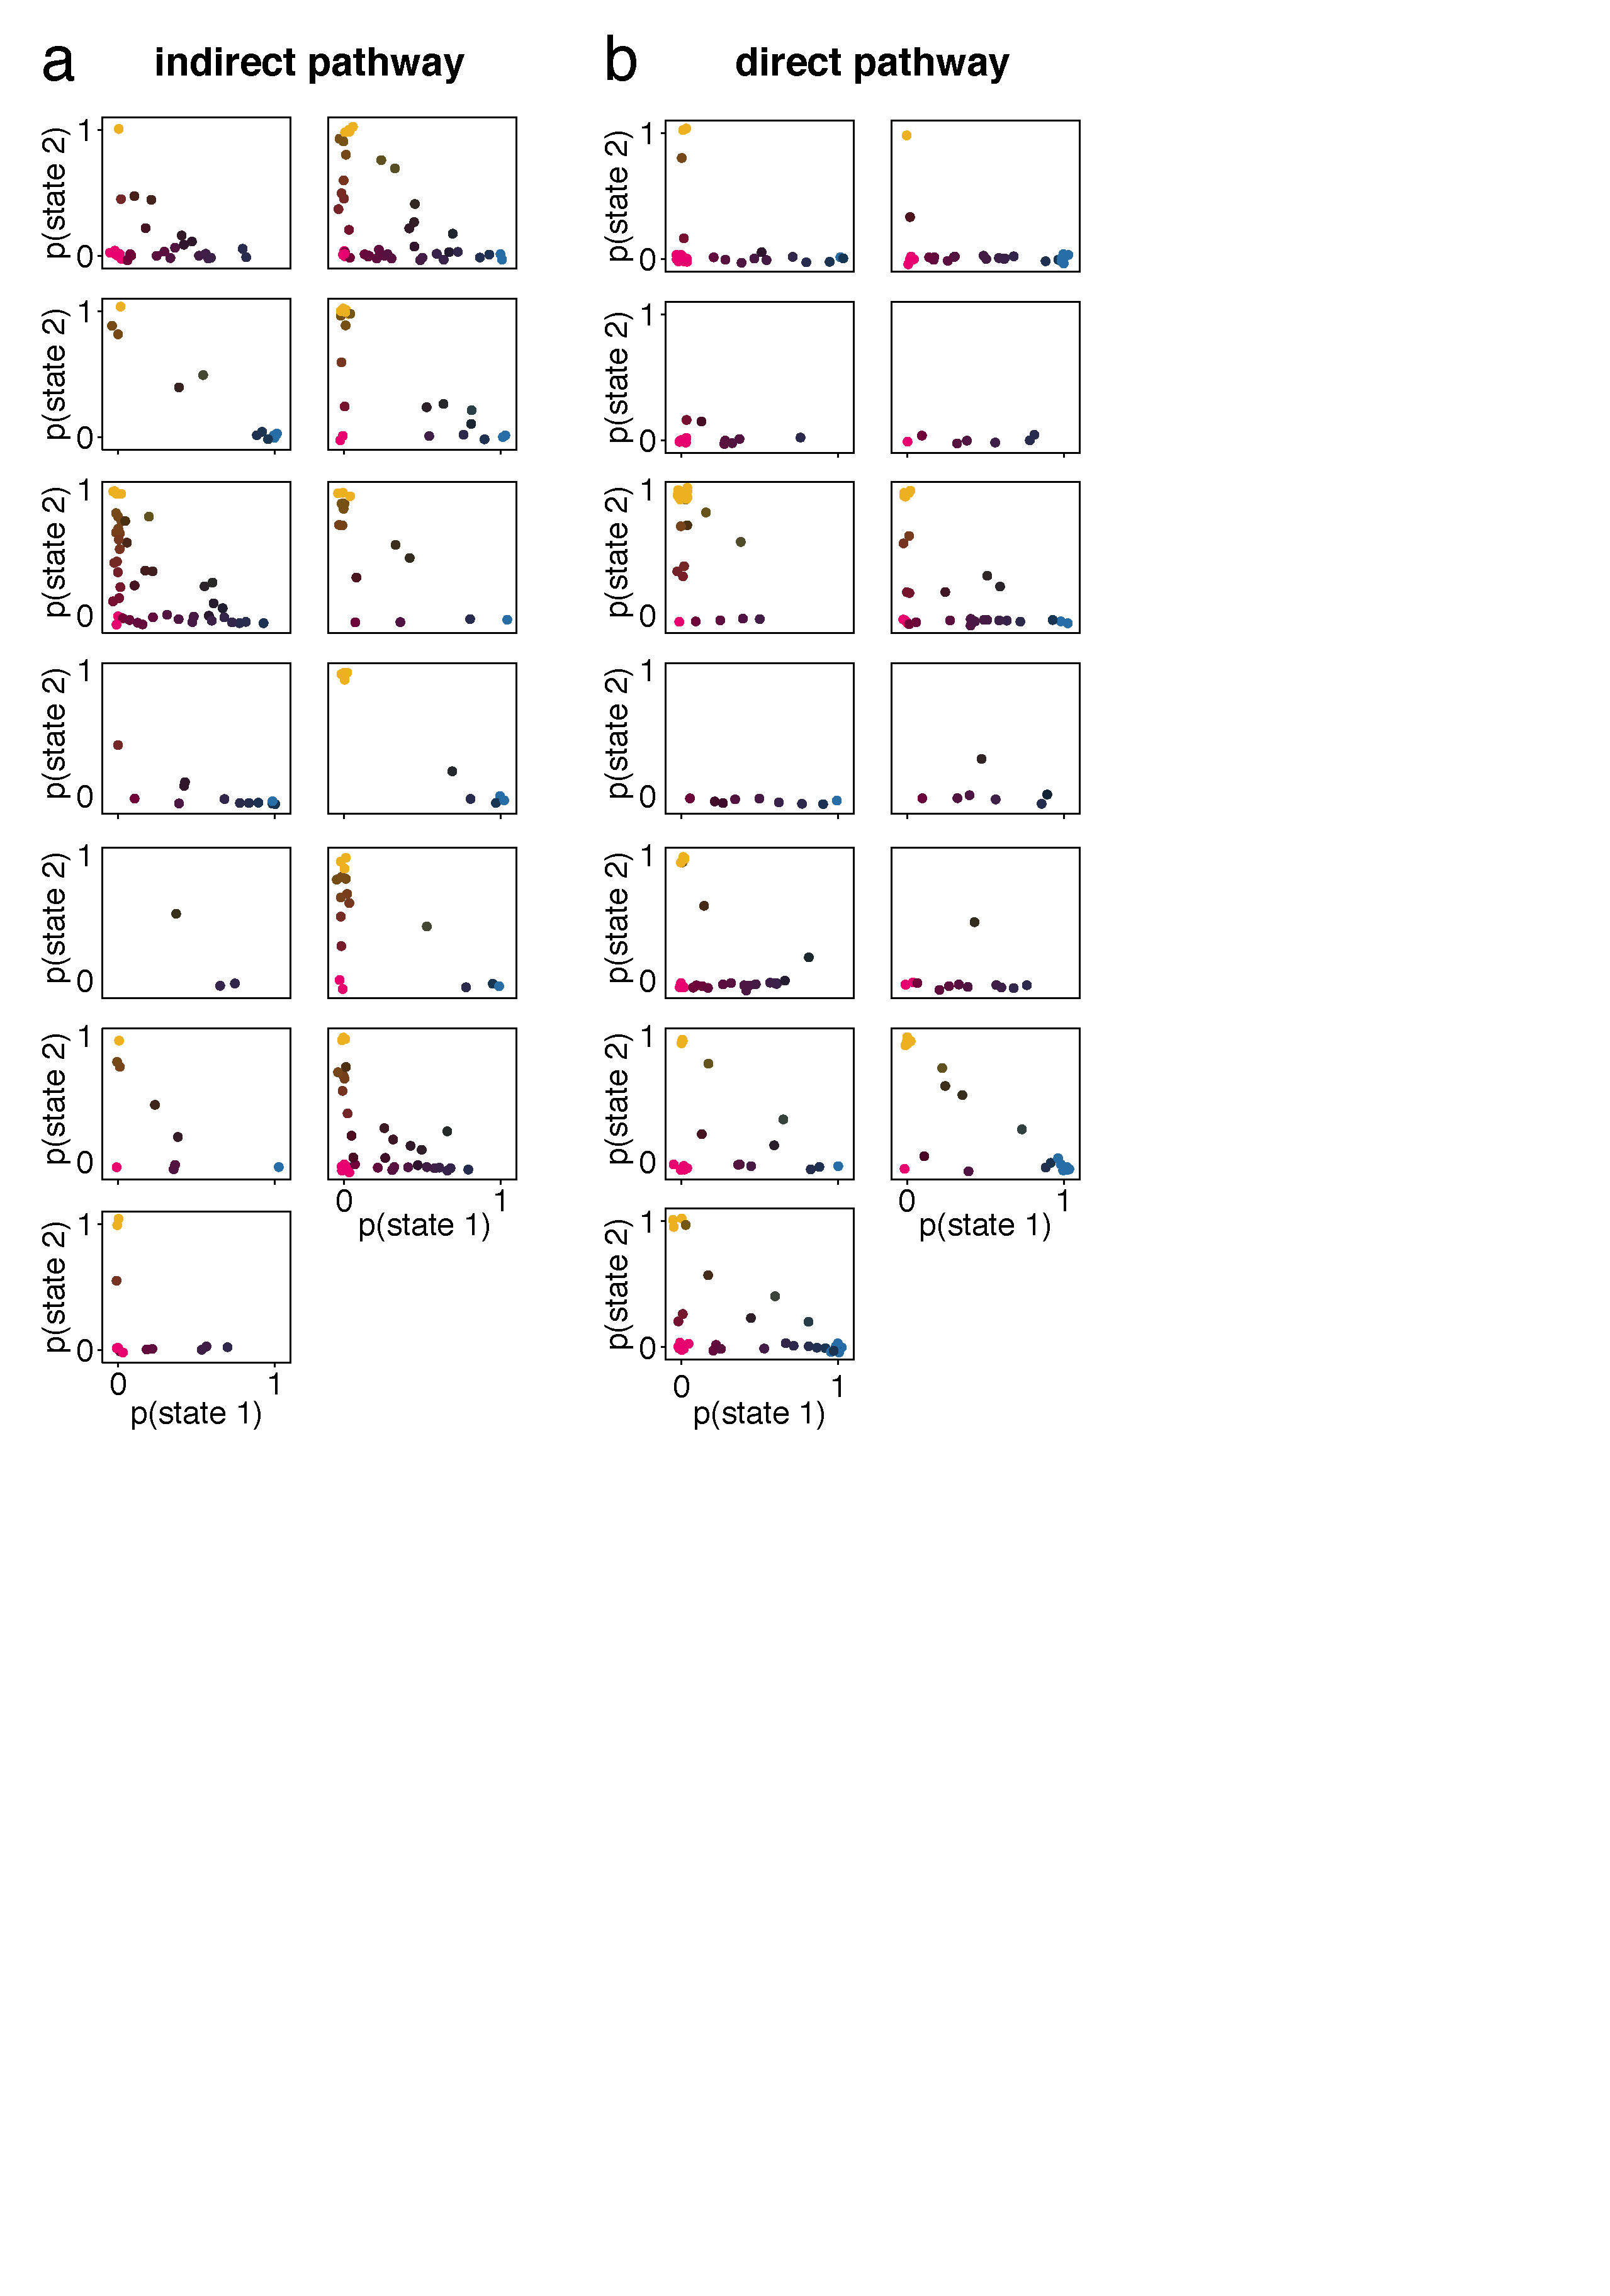
\includegraphics[width=0.70\linewidth]{ch7-appendix1/appendix1-figures/Supplementary_Fig4.pdf}
    \caption[Individual mice visit multiple types and numbers of states over the course of sessions]{\textbf{Individual mice visit multiple types and numbers of states over the course of sessions.} (a) The fraction of trials that mice inhibited in the indirect pathway of the DMS spent in each state in each session. Each box represents a different mouse (n=13) and each dot in each box represents an individual session for that mouse. Color-coding reinforces the state composition of each session (e.g. blue indicates the mouse spent 100\% of the session in state 1). A small amount of Gaussian noise was added to the position of each dot for visualization purposes. (b) Same as A but for mice inhibited in the direct pathway of the DMS (n=13).}
    \label{fig:ap1:supp4}
  \end{center}
  %\vspace{-1.5cm}
\end{figure}
\begin{figure}[t!]
%\vspace{-2.5cm}
  \begin{center}
    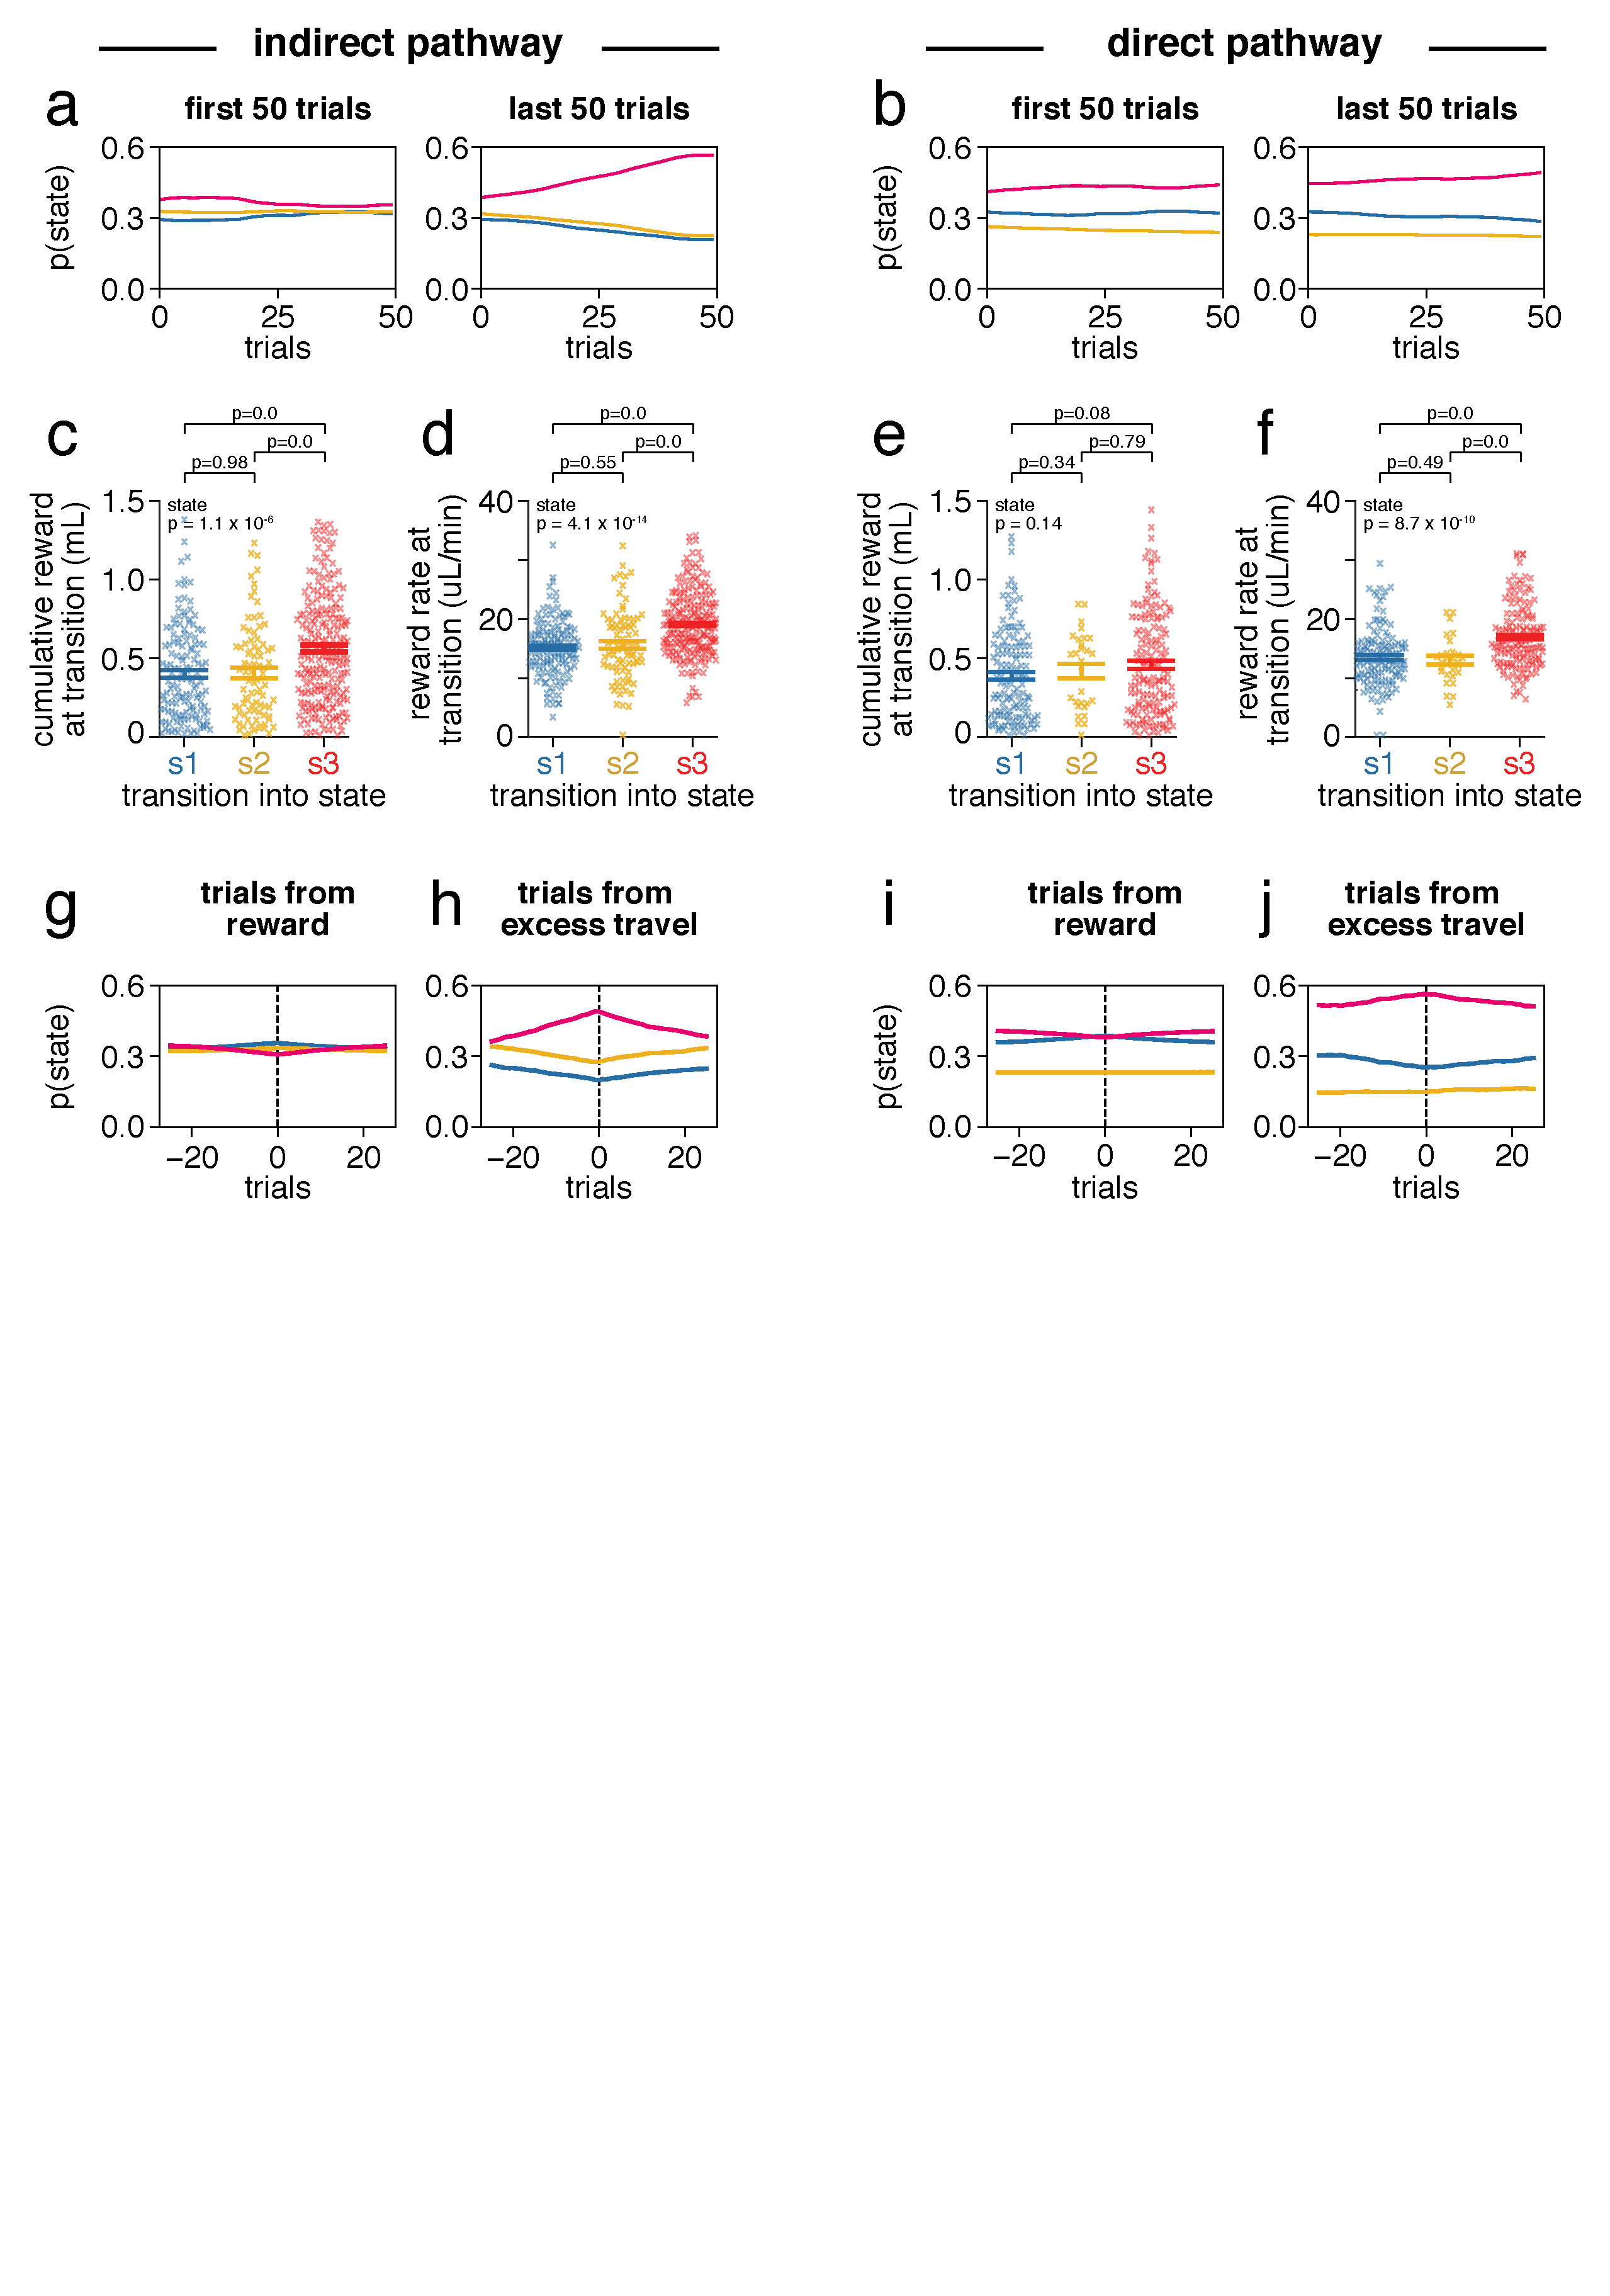
\includegraphics[width=0.90\linewidth]{ch7-appendix1/appendix1-figures/ExtData_Fig8.pdf}
    \caption[GLM-HMM state 3 is associated with indicators of task disengagement]{\textbf{GLM-HMM state 3 is associated with indicators of task disengagement.} (a) The mean posterior probability of each state over the first and last 50 trials of a session, averaged across all sessions for mice inhibited in the indirect pathway of the DMS (n=271 sessions). (b) Same as a but for mice receiving DMS direct pathway inhibition (n=266 sessions). (c) Mean $\pm$ S.E.M. of the cumulative reward received in a session prior to transitions into state 1 (n = 142), state 2 (n = 85), or state 3 (n = 237) in indirect pathway mice. One-way ANOVA of transition state on cumulative reward (p = 1.0 x 10-6; F2,460 = 14.2). Unpaired, two-tailed Wilcoxon ranksum comparison between transition types (state 1 vs 2: p = 0.96, z = -0.03; state 2 vs 3: p = 0, z = -3.6; state 1 vs 3: p = 0, z = -4.5). (d) Mean $\pm$ S.E.M. of the reward rate (uL/min) in a session prior to transitions into each state for indirect pathway mice. Reward rate was calculated as the sum of reward received from the start of the session up to the transition trial divided by the sum of the duration of all trials from the start of the session up to the transition trial. One-way ANOVA of transition state on reward rate (p = 4.1 x 10-14; F2,460 = 32.9). Unpaired, two-tailed Wilcoxon ranksum comparison between transition types (state 1 vs 2: p = 0.55, z = -0.6; state 2 vs 3: p = 0, z = -4.9; state 1 vs 3: p = 0, z = -7.4). (e) Same as c but for direct pathway mice (state 1: n = 140; state 2: n = 29; state 3: n = 159). One-way ANOVA of transition state on cumulative reward (p = 0.14; F2,325 = 1.99). Unpaired, two-tailed Wilcoxon ranksum comparison between transition types (state 1 vs 2: p = 0.35, z = -0.9; state 2 vs 3: p = 0.78, z = -0.27; state 1 vs 3: p = 0.08, z = -1.74). (f) Same as d but for direct pathway mice. One-way ANOVA of transition state on reward rate (p = 8.7 x 10-10; F2,325 = 22.6). Unpaired, two-tailed Wilcoxon ranksum comparison between transition types (state 1 vs 2: p = 0.49, z = 0.69; state 2 vs 3: p = 0.0, z = -4.2; state 1 vs 3: p = 0.0, z = -5.9). (g) The mean posterior probability of each state aligned $\pm$ 25 trials to}
    \label{fig:ap1:ext8}
  \end{center}
  %\vspace{-1.5cm}
\end{figure}
\begin{figure}[t!]
%\vspace{-3cm}
  \contcaption{to trials in which reward was received for indirect pathway mice. (h) Same as g but state probability aligned to trials with excess travel (defined as 10\% greater than the maze stem, or 330cm). (i) Same as g but for direct pathway mice. (j) Same as h but for direct pathway mice.}% Continued caption
\end{figure}
\begin{figure}[t!]
\vspace{-0.2cm}
  \begin{center}
    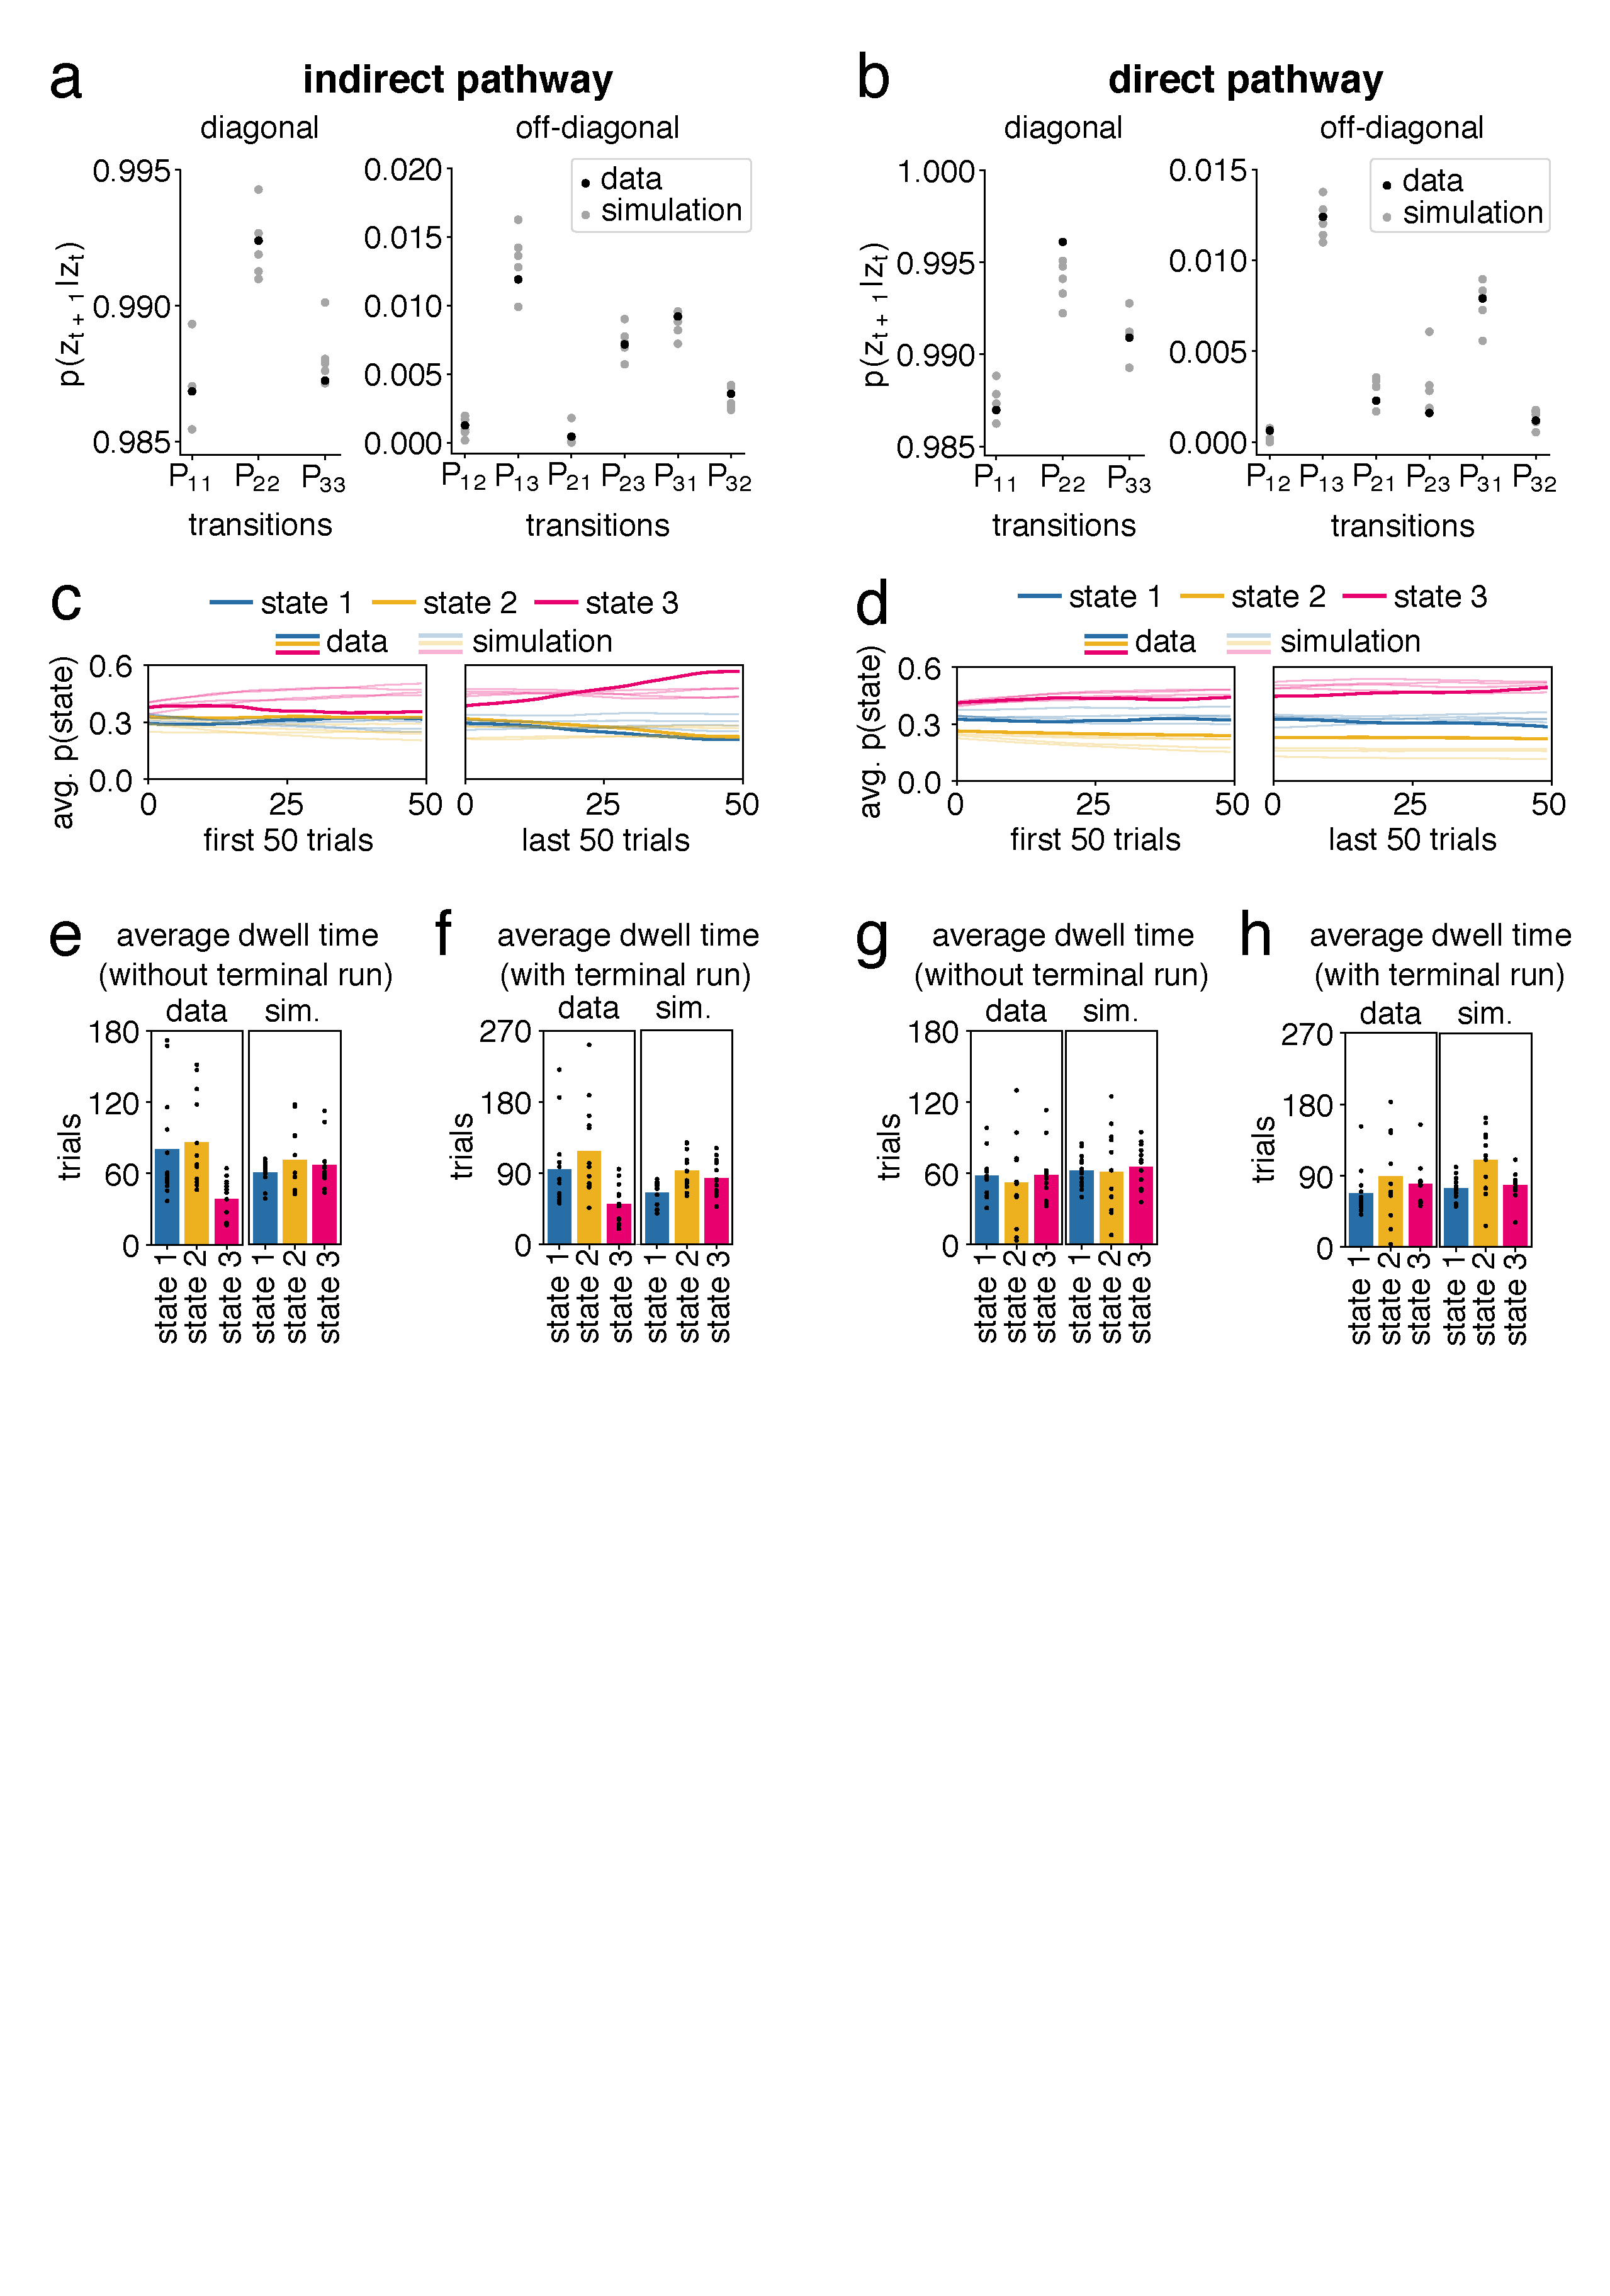
\includegraphics[width=0.90\linewidth]{ch7-appendix1/appendix1-figures/ExtData_Fig9.pdf}
    \caption[Model simulations recapitulate transition and state characteristics of real data]{\textbf{Model simulations recapitulate transition and state characteristics of real data.} (a) Transition probabilities of the model fit to data from mice inhibited in the DMS indirect pathway (black) and from five simulated datasets generated from the model fit to mice inhibited in the indirect pathway of the DMS (gray), shown separately for diagonal (left) and off-diagonal (right) probabilities. (b) Same as a but for mice inhibited in the direct pathway of the DMS. (c) The posterior probability of each state over the first and last 50 trials of a session, averaged across all sessions for mice inhibited in the indirect pathway of the DMS (n=271). Dark lines denote average for real data (same as Fig. 7E) and faded lines indicate averages for each of the five simulations. (d) Same as c but for mice inhibited in the direct pathway of the DMS (dark lines are the same as shown in Fig. 7F). (e) Dwell times showing the average consecutive number of trials that mice inhibited in the DMS indirect pathway spent in each state for real data (left; range 39-86 trials, average session length 202 trials, same as shown in Fig. 7g) and one simulated dataset (right; range 60-71 trials, average session length 202 trials). Black dots show averages for individual mice (n=13). We removed the last run in each session (including any run that lasted the entire session length) from the analysis, as the termination of the session prematurely truncated the length of }
    \label{fig:ap1:ext9}
  \end{center}
  %\vspace{-1.5cm}
\end{figure}
\begin{figure}[t!]
%\vspace{-3cm}
  \contcaption{those runs. (f) Same as e but without removing the last run in each session for real data (left; range 51-118 trials, average session length 202 trials) and one simulated dataset (right; range 65-93 trials, average session length 202 trials). (g) Same as e but for mice inhibited in the direct pathway of the DMS for real data (left; range 52-59 trials, average session length 185 trials, same as shown in Fig. 7g) and one simulated dataset (right; range 61-66 trials, average session length 185 trials). Black dots show averages for individual mice (n=13). (h) Same as g but without removing the last run in each session for real data (left; 67-89 trials, average session length 185 trials) and one simulated dataset (right; range 74-110 trials, average session length 185 trials).}% Continued caption
\end{figure}
\begin{figure}[t!]
\vspace{-0.2cm}
  \begin{center}
    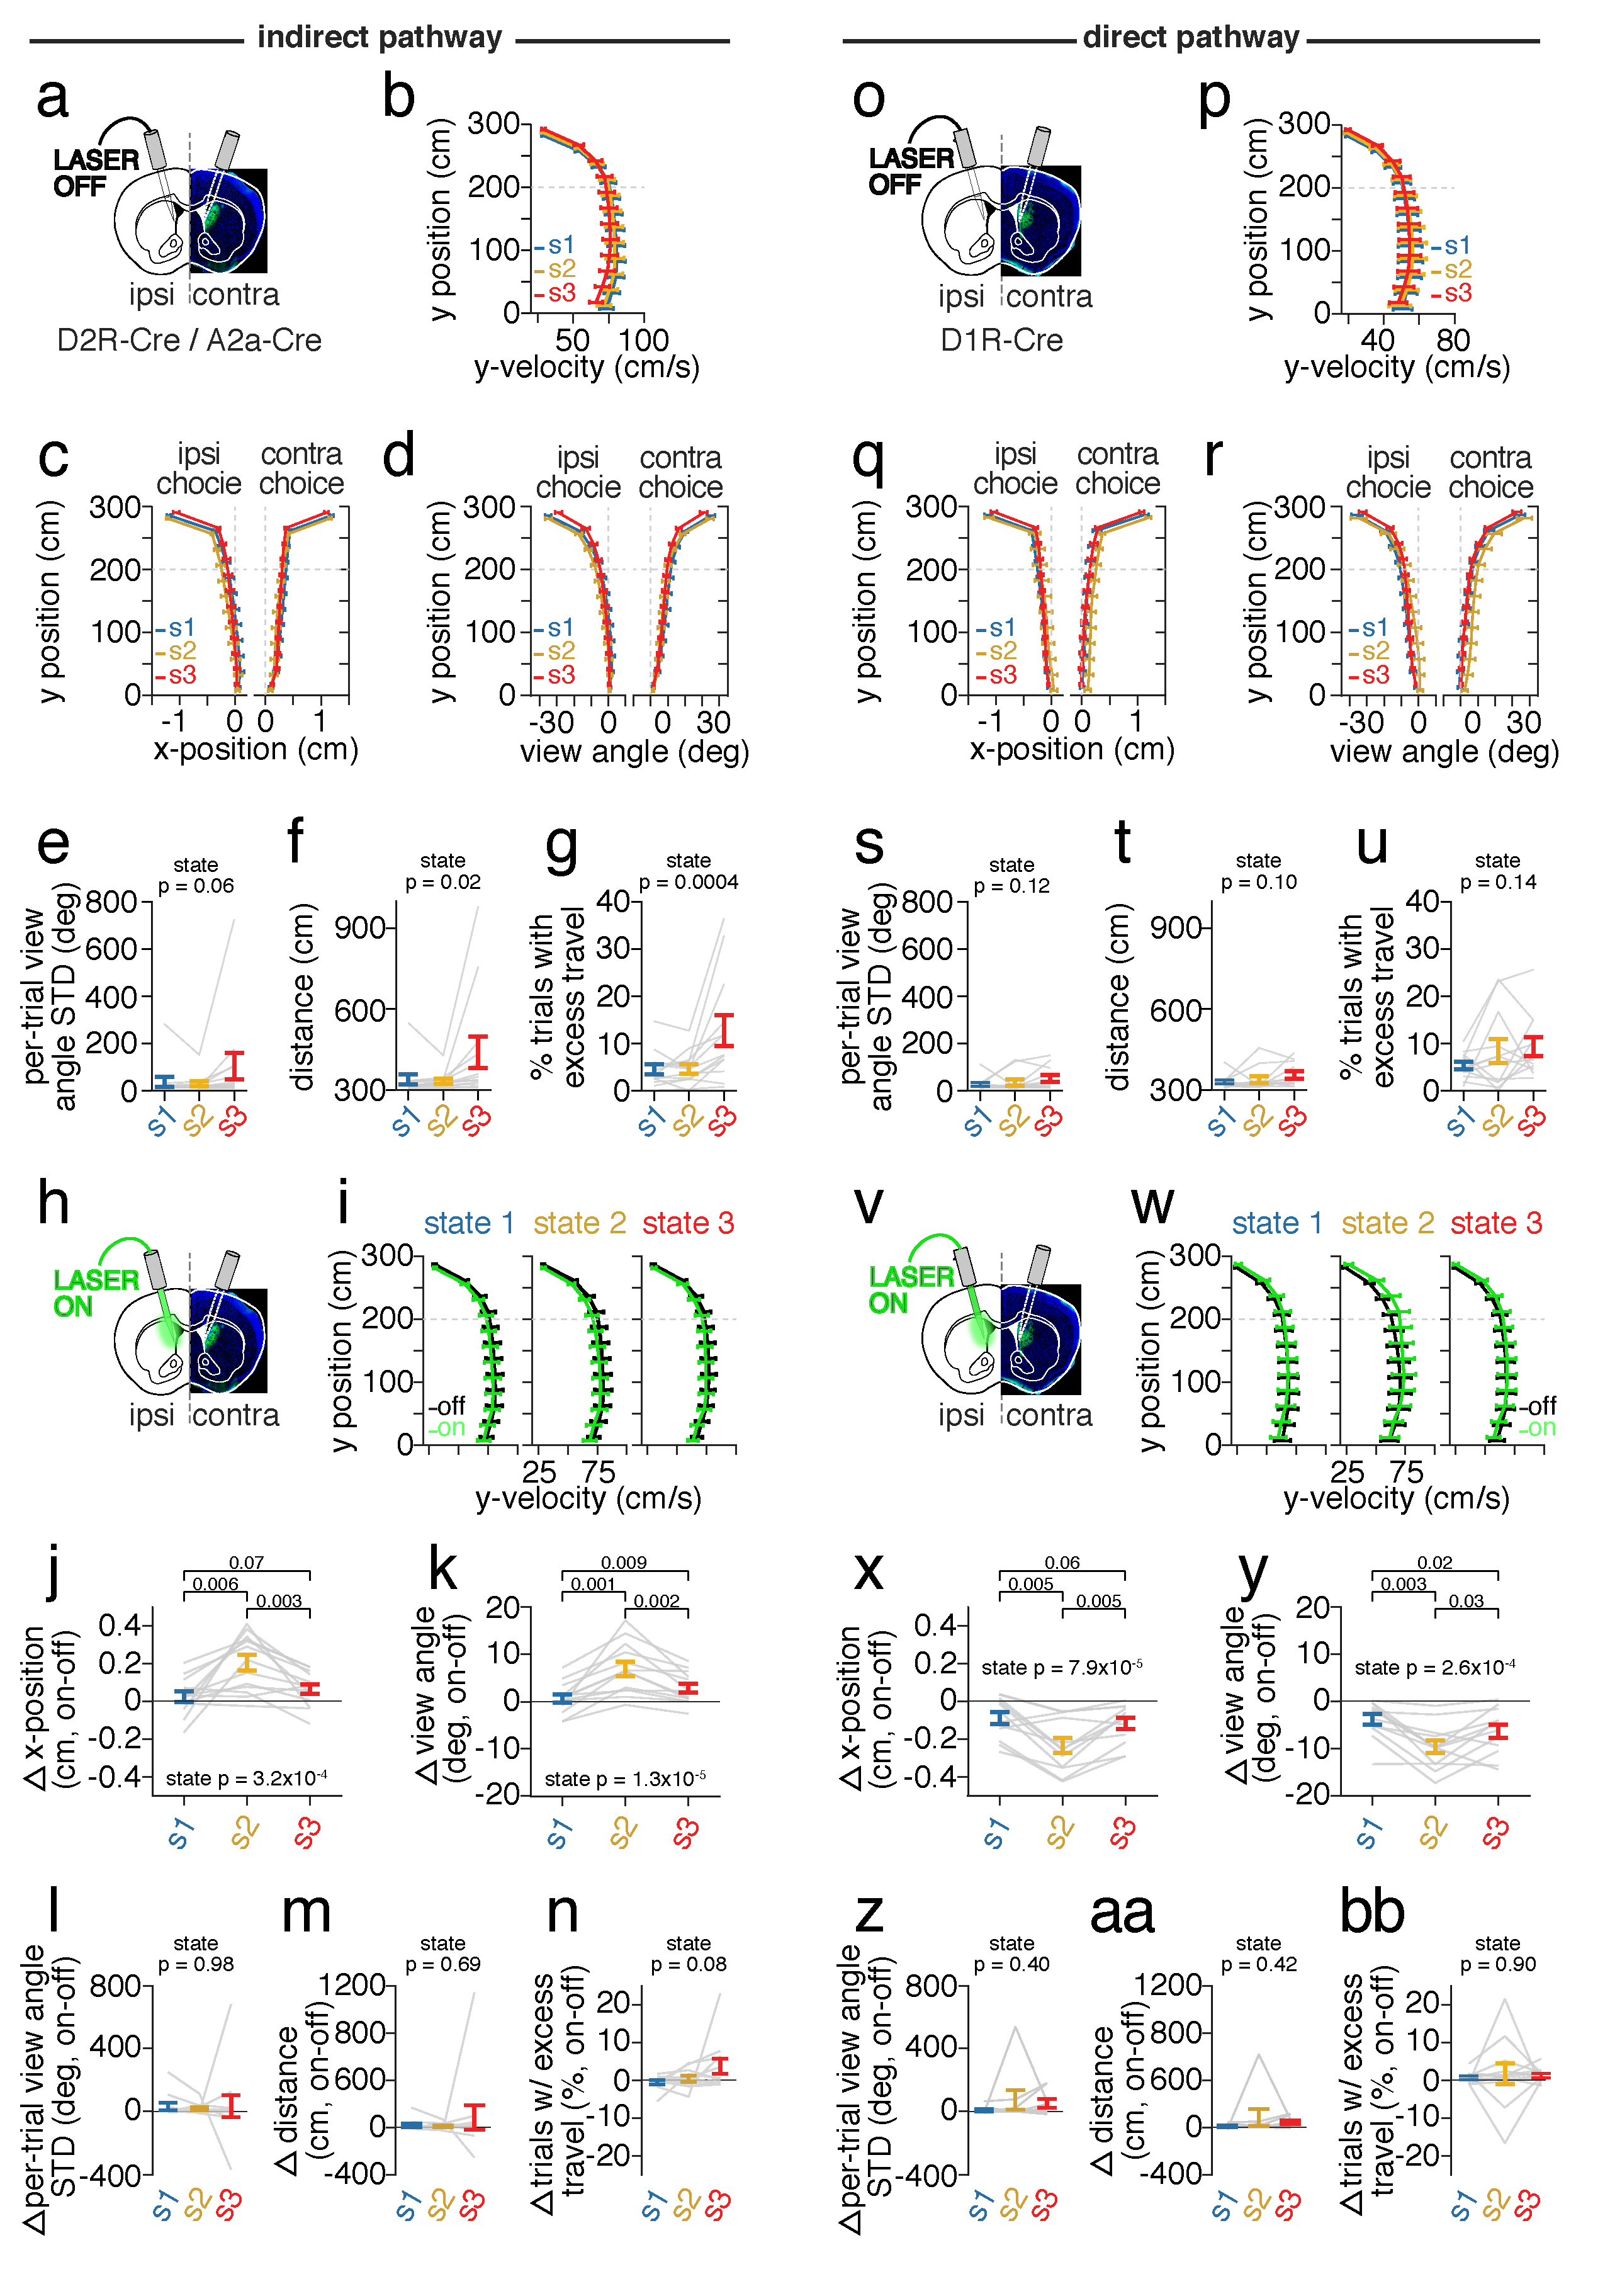
\includegraphics[width=0.90\linewidth]{ch7-appendix1/appendix1-figures/ExtData_Fig10.pdf}
    \caption[Comparison of motor performance across GLM-HMM states with and without pathway-specific DMS inhibition]{\textbf{Comparison of motor performance across GLM-HMM states with and without pathway-specific DMS inhibition.} }
    \label{fig:ap1:ext10}
  \end{center}
  %\vspace{-1.5cm}
\end{figure}
\begin{figure}[t!]
%\vspace{-3cm}
  \contcaption{(a) Schematic denoting analysis of motor performance across GLM-HMM states on laser off trials only (panels b-g) in mice unilaterally coupled to a fiberoptic for indirect pathway inhibition. (b) Average y-velocity (cm/s) during laser off trials as a function of y-position in the maze (0-300 cm in 25-cm bins) in indirect pathway mice across GLM-HMM states (state 1, blue: n = 13,394 trials; state 2, yellow: n = 13,570 trials; state 3, red: n = 16,982 trials). (c) As in b but for average x-position (cm) on ipsilateral or contralateral choice trials (n as in b). (d) As in c but for average view angle (degrees) on ipsilateral and contralateral choice trials (n as in b). (e) Mean per-trial standard deviation in view angle during laser off trials across GLM-HMM states (state 1, blue: n = 13,854 trials; state 2, yellow: n = 14,201 trials; state 3, red: n = 18,258 trials). p-value denotes one-way repeated measures ANOVA of state on view angle deviation (p = 0.06, F2,24 = 3.2). (f) As in e but for average distance traveled (cm) per trial. p-value denotes one-way repeated measures ANOVA of state on distance (p = 0.02, F2,24 = 5.0, n as in e). (g) As in e but for average percent of trials with excess travel. p-value denotes one-way repeated measures ANOVA of state on excess travel (p = 0.0004, F2,24 = 10.9, n as in e). (h) Schematic denoting analysis of effects of indirect pathway DMS inhibition on motor performance across GLM-HMM states in i-n. (i) As in b but for average y-velocity on laser off (black) or laser on (green) trials across GLM-HMM states (n of laser off trials as in b-g, n of laser on trials: state 1, blue: n = 2,302 trials; state 2, yellow: n = 1,858 trials; state 3, red: n = 3,005 trials). (j) As in c but for delta (on-off) x-position (cm) during the cue region (0-200cm) across GLM-HMM states in mice with indirect pathway inhibition . p-value denotes one-way repeated measures ANOVA of state on delta x-position (p = 3.2x10-4, F2,24 = 11.4, n as in i). Post-hoc comparisons reflect two-tailed, paired Willcoxon signed rank tests between states (state 1 vs state 3: p = 0.07, z = 1.7; state 1 vs state 2: p = 0.006, z = 2.7; state 2 vs state 3: p = 0.03, z = 2.4). (k) As in j but for delta (on-off) view angle (degrees). p-value denotes one-way repeated measures ANOVA of state on delta view angle (p = 1.2x10-5, F2,26 = 18.7, n as in i). Post-hoc comparisons reflect two-tailed, paired Willcoxon signed rank tests between states (state 1 vs state 3: p = 0.009, z = 2.6; state 1 vs state 2: p = 0.001, z = -3.18; state 2 vs state 3: p = 0.002, z = -3.1). (l) Same as e but for delta (on-off) mean per-trial view angle standard deviation across GLM-HMM states in mice with indirect pathway inhibition (n of laser off trials as in e-g, n of laser on trials: state 1, blue: n = 2,887 trials; state 2, yellow: n = 2,713 trials; state 3, red: n = 2,970 trials). p-value denotes one-way repeated measures ANOVA of state on delta view angle deviation (p = 0.97, F2,24 = 0.03, n as in l). (m) Same as f but for delta (on-off) in mean per-trial distance (cm) traveled across GLM-HMM states with indirect pathway inhibition (p = 0.68, F2,24 = 0.38, n as in l). (n) Same as g but for delta (on-off) in percent of trials with excess travel across GLM-HMM states with direct pathway inhibition (p = 0.08, F2,24 = 2.8, n as in l). (o) As in a but schematic denoting analysis of motor performance across GLM-HMM states on laser off trials only in mice unilaterally coupled to a fiberoptic for direct pathway inhibition in p-u. (p) As in b but for y-velocity (cm/s) on laser off trials across GLM-HMM states in direct pathway mice (state 1, blue: n = 12,294 laser off and n = 2,302 laser on trials; state 2, yellow: n = 9,201 laser off and n = 1,858 laser on trials; state 3, red: n = 16,239 laser off and n = 3,005 laser on trials). (q) As in c but x-position (cm) for direct pathway mice (n as in p). (r) As in d but for view angle (degrees) for direct pathway mice (n as in p). (s) As in e but for mean per-trial view angle standard deviation across GLM-HMM states in direct pathway mice (state 1, blue: n = 13,403 laser off and n = 2,508 laser on trials; state 2, yellow: n = 9,555 laser off and n = 1,969 laser on trials; state 3, red: n = 18,292 laser off and n = 3,450 laser on trials). p-value denotes one-way repeated measures ANOVA of state on per-trial view angle standard deviation (p = 0.12, F2,24 = 2.3). (t) As in f but for distance (cm) in direct pathway mice (p = 0.1, F2,24 = 2.5). }% Continued caption
\end{figure}
\begin{figure}[t!]
%\vspace{-3cm}
  \contcaption{(u) As in g but for percent trials with excess travel in direct pathway mice (p = 0.14, F2,24 = 2.1). (v) As in h but schematic denoting analysis of effects of direct pathway DMS inhibition on motor performance across GLM-HMM states in w-bb. (w) As in i but for the mean y-velocity (cm/s) on laser on (green) and off (black) trials across GLM-HMM states in direct pathway mice. (x) As in j but for the delta (on-off) x-position (cm) across GLM-HMM states in direct pathway mice. p-value denotes one-way repeated measures ANOVA of state on delta x-position (p = 7.9x10-5, F2,24 = 14.9). Posthoc comparisons reflect two-tailed, paired Willcoxon signed rank tests between states (state 1 vs state 3: p = 0.06, z = 1.8; state 1 vs state 2: p = 0.005, z = 2.8; state 2 vs state 3: p = 0.005, z = 2.8). (y) As in k but for delta (on-off) view angle (degrees) across GLM-HMM states in direct pathway mice. p-value denotes one-way repeated measures ANOVA of state on delta view angle (p = 2.6x10-4, F2,24 = 12.3). Posthoc comparisons reflect two-tailed, paired Willcoxon signed rank tests between states (state 1 vs state 3: p = 0.03, z = 2.3; state 1 vs state 2: p = 0.003, z = 2.98; state 2 vs state 3: p = 0.03, z = 2.1). (z) As in l but for delta (on-off) mean per-trial view angle standard deviation (degrees) in direct pathway mice (p = 0.40, F2,24 = 0.94, n as in s-u). (aa) as in m but for delta (on-off) in mean distance (cm) traveled in direct pathway mice (p = 0.43, F2,24 = 0.89). (bb) as in n but for delta (on-off) in percent trials with excess travel in direct pathway mice (p = 0.90, F2,24 = 0.1). Throughout solid colored bars denote mean $\pm$ S.E.M. while transparent grey lines reflect individual mouse mean.}% Continued caption
\end{figure}
\begin{figure}[t!]
\vspace{-0.2cm}
  \begin{center}
    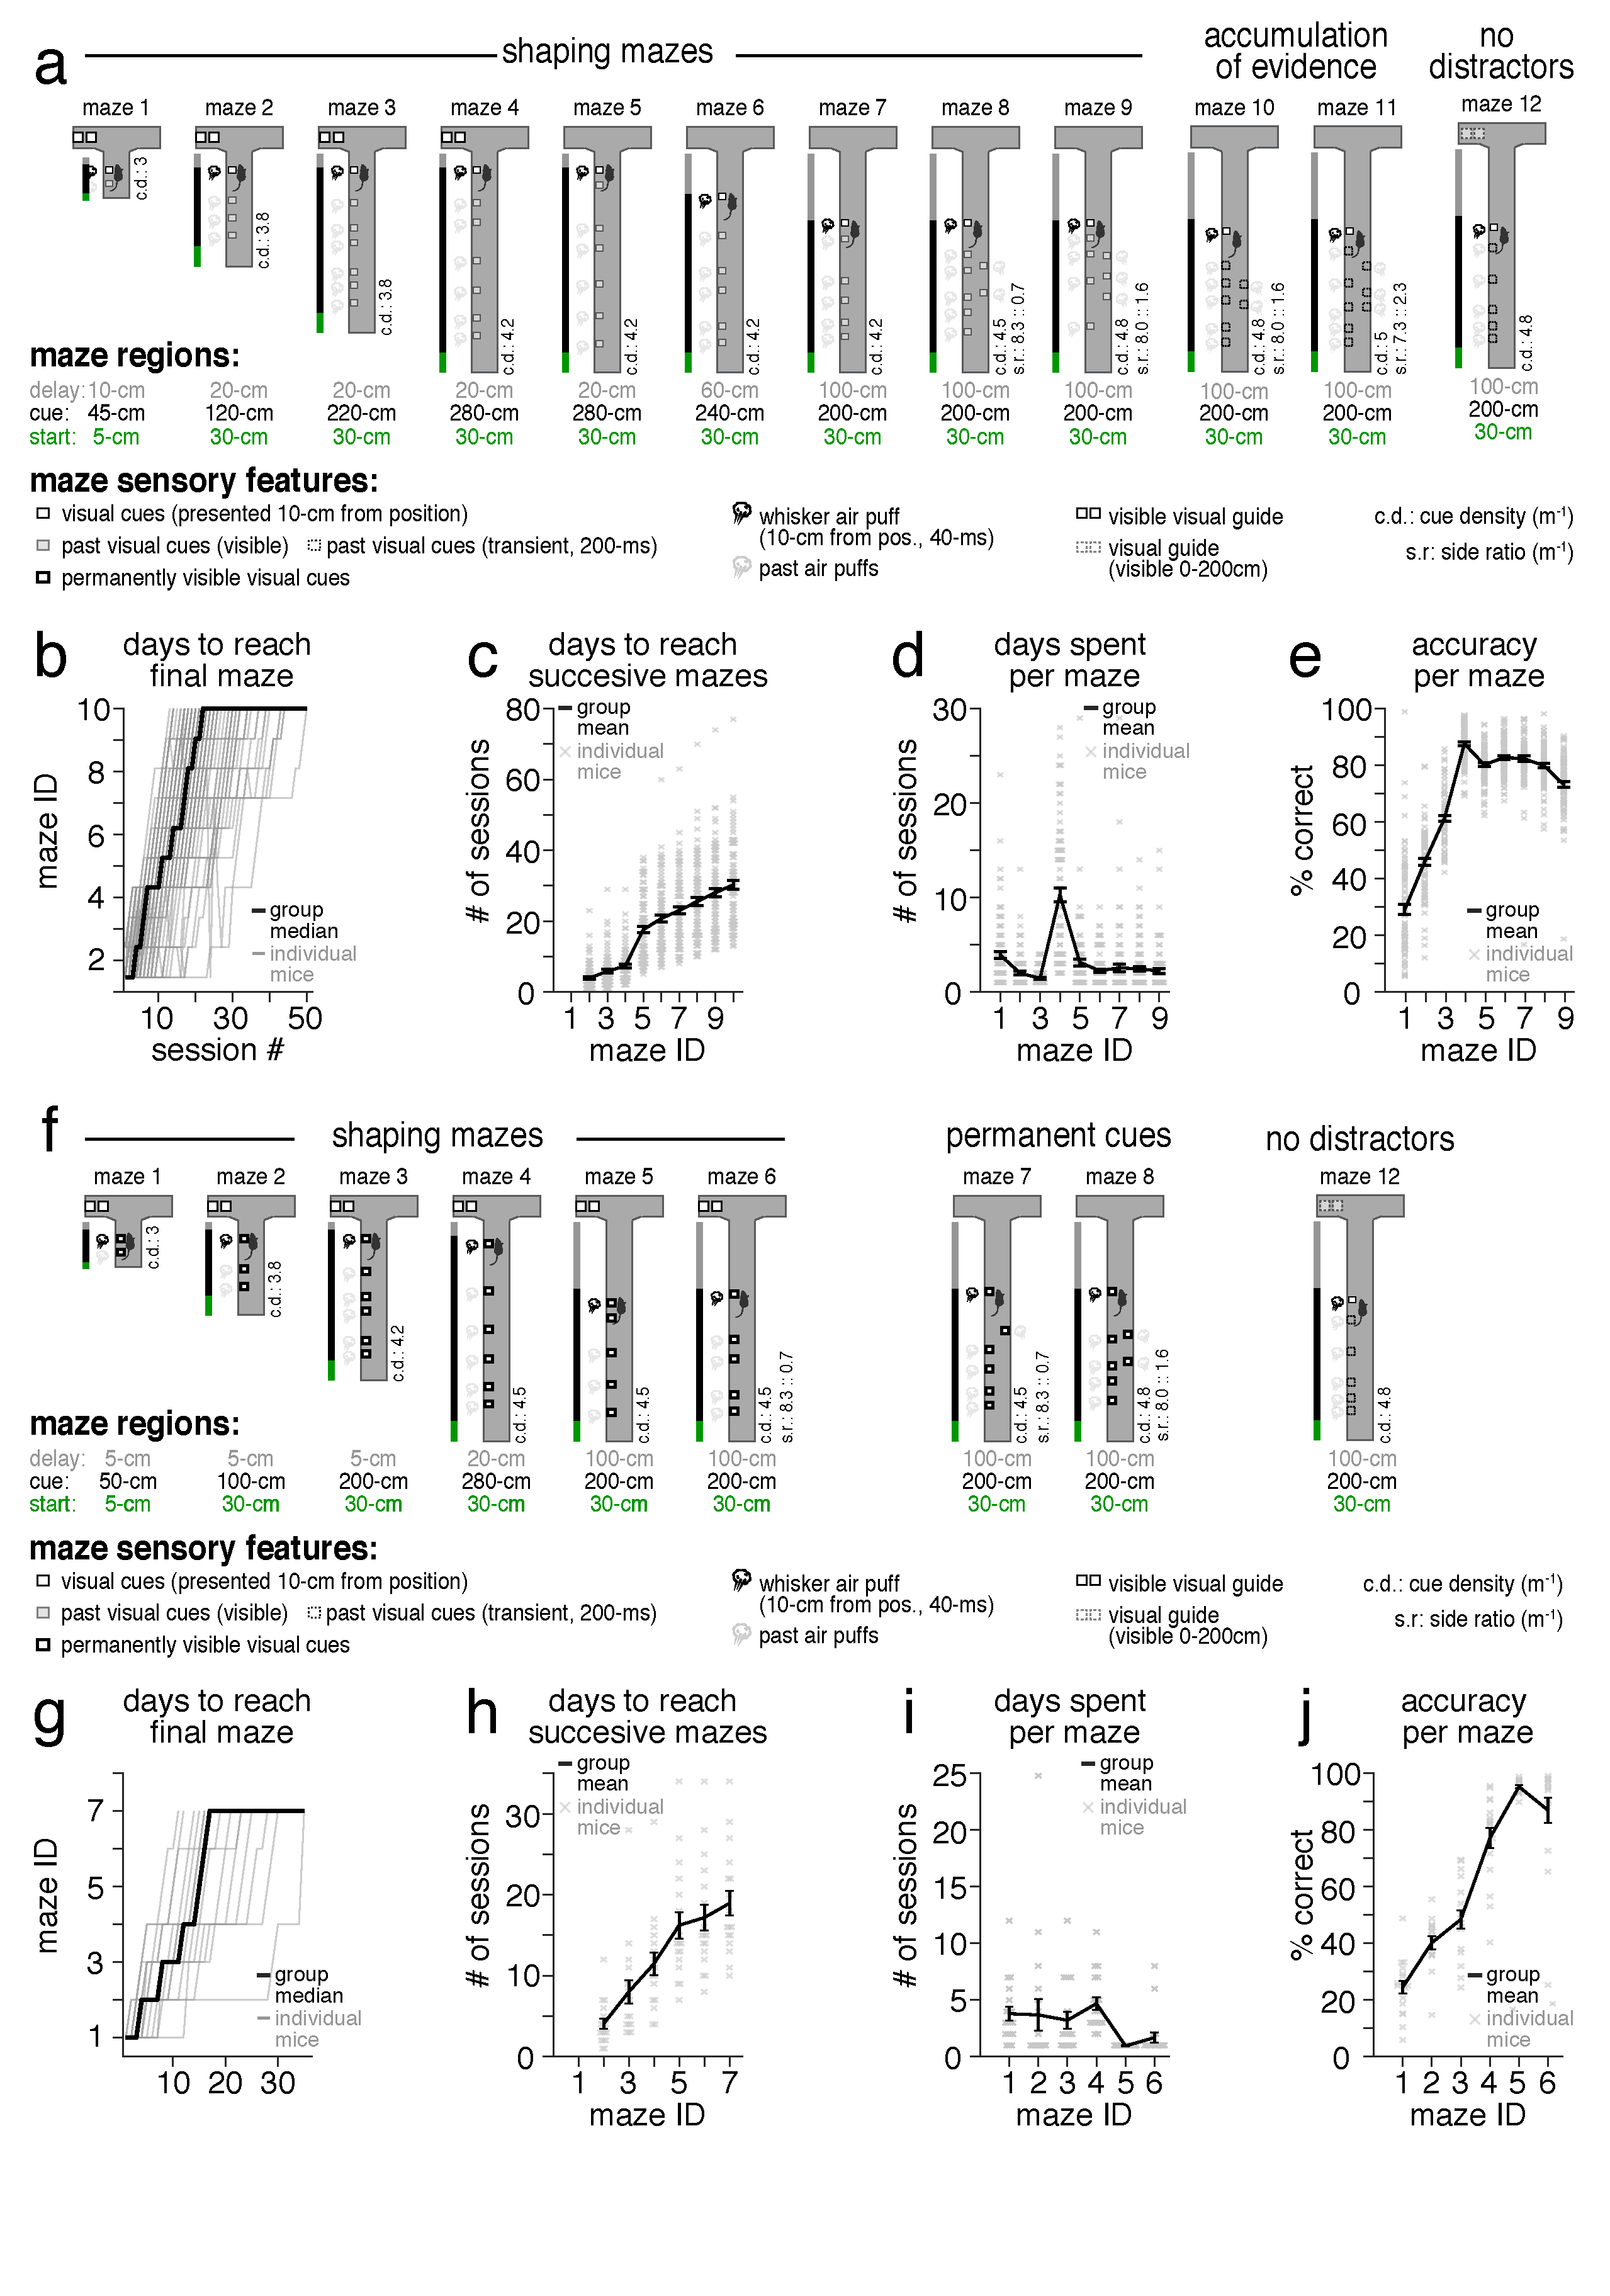
\includegraphics[width=0.90\linewidth]{ch7-appendix1/appendix1-figures/Supplementary_Fig5.pdf}
    \caption[Behavioral shaping for virtual-reality T-maze tasks]{\textbf{Behavioral shaping for virtual-reality T-maze tasks.} }
    \label{fig:ap1:supp5}
  \end{center}
  %\vspace{-1.5cm}
\end{figure}
\begin{figure}[t!]
\vspace{-9cm}
  \contcaption{(a) Schema of shaping mazes (top: maze 1-9) and subsequent optogenetic testing mazes (far right) for the accumulation of evidence task. Mazes varied according to the following sensory features: the length of start, cue, and delay regions (green, black, and grey bars and colored text, respectively), whether visual cues were presented 10-cm from cue position (black outline, white filled square) and  remained visible (grey square) or disappeared 200-ms after presentation (black dotted, unfilled square) or were permanently available from trial outset (bold black border, white filled), the presence of left or right whisker air puffs (15-psi, 40-ms) which were delivered upon first instance of being 10-cm from visual cue position (solid vs grey puff symbol), whether a visual guide was located in the rewarded arm (black double square) or if the visual guide was only visible during the cue region (grey double square), the density of cues during the cue region (c.d.), and whether distractor cues occurred on the non-rewarded maze side (side ratio, s.r.: mean density per meter). Following shaping mazes 1-9, optogenetic testing was carried out on mazes 10 and 11 (accumulation of evidence), and maze 12 (no distractors). (b) Solid black line depicts the across-mouse median number of sessions spent on each shaping maze (mazes 1-9) until reaching the first testing maze (maze 10) (group median: 22 sessions). Grey transparent lines depict the median number of sessions for individual mice (n = 79). (c) Cumulative number of sessions to reach each successive maze until the first testing maze (maze 10) (group mean: 23.0 $\pm$ 0.8 sessions). Solid black lines depict mean and s.e.m. across mice, and transparent ‘x’ denote individual mice. (d) Total number of sessions spent on each shaping maze. Solid black lines depict mean and s.e.m., and transparent ‘x’ denote individual mice at each respective shaping maze (maze 1-9). (e) Percent correct performance across shaping mazes. Solid black lines depict mean and s.e.m., and transparent ‘x’ denote individual mice at each respective shaping maze (maze 1-9). (f) Same as a but for shaping (left, maze 1-6) for the permanent cues task. Following shaping mazes 1-6, optogenetic testing was carried out on mazes 7 and 8 (permanent cues) and maze 12 (no distractors). (g) Same as b but for permanent cues shaping (group median: 17 days; n = 20 mice). (h) Same as c but for permanent cues shaping (group mean: 18.9 $\pm$ 1.5 sessions). (i) Same as d but for permanent cues shaping. (j) Same as e but for permanent cues shaping. }% Continued caption
\end{figure}
\begin{figure}[t!]
\vspace{-1cm}
  \begin{center}
    \includegraphics[width=0.80\linewidth]{ch7-appendix1/appendix1-figures/Supplementary_Fig6.pdf}
    \caption[Histological confirmation of viral expression and fiberoptic placement]{\textbf{Histological confirmation of viral expression and fiberoptic placement.} (A) Top: two individual mouse examples of cre-dependent NpHR-GFP expression in and fiberoptic targeting of the dorsomedial striatum (DMS) in D2R-Cre or A2a-Cre mice. Bottom left: schematic representation of the minimum (dark grey) and maximum (light grey) spread of NpHR expression in all mice targeting the indirect pathway of the DMS (DMS::Indirect, n = 21 mice). Bottom right: summary of tapered fiberoptic tip location and angled track for all mice targeting the indirect pathway of the DMS. (B) Same as A but for all experiments targeting the direct pathway of the DMS (DMS::Direct, n = 23 mice). (C) Same as A but for fiberoptic targeting only for all control mice receiving DMS illumination in the absence of NpHR (DMS::NoOpsin, n = 17 mice). (D) Same as A but for experiments targeting the indirect pathway of the nucleus accumbens (NAc::Indirect, n = 9 mice). (E) Same as A but for experiments targeting the direct pathway of the nucleus accumbens (NAc::Direct, n = 10 mice). (F) Same as C but for all control mice receiving NAc illumination in the absence of NpHR (NAc::NoOpsin, n = 7). }
    \label{fig:ap1:supp6}
  \end{center}
  %\vspace{-1.5cm}
\end{figure}